\documentclass[twoside]{book}

% Packages required by doxygen
\usepackage{fixltx2e}
\usepackage{calc}
\usepackage{doxygen}
\usepackage[export]{adjustbox} % also loads graphicx
\usepackage{graphicx}
\usepackage[utf8]{inputenc}
\usepackage{makeidx}
\usepackage{multicol}
\usepackage{multirow}
\PassOptionsToPackage{warn}{textcomp}
\usepackage{textcomp}
\usepackage[nointegrals]{wasysym}
\usepackage[table]{xcolor}

% Font selection
\usepackage[T1]{fontenc}
\usepackage[scaled=.90]{helvet}
\usepackage{courier}
\usepackage{amssymb}
\usepackage{sectsty}
\renewcommand{\familydefault}{\sfdefault}
\allsectionsfont{%
  \fontseries{bc}\selectfont%
  \color{darkgray}%
}
\renewcommand{\DoxyLabelFont}{%
  \fontseries{bc}\selectfont%
  \color{darkgray}%
}
\newcommand{\+}{\discretionary{\mbox{\scriptsize$\hookleftarrow$}}{}{}}

% Page & text layout
\usepackage{geometry}
\geometry{%
  a4paper,%
  top=2.5cm,%
  bottom=2.5cm,%
  left=2.5cm,%
  right=2.5cm%
}
\tolerance=750
\hfuzz=15pt
\hbadness=750
\setlength{\emergencystretch}{15pt}
\setlength{\parindent}{0cm}
\setlength{\parskip}{3ex plus 2ex minus 2ex}
\makeatletter
\renewcommand{\paragraph}{%
  \@startsection{paragraph}{4}{0ex}{-1.0ex}{1.0ex}{%
    \normalfont\normalsize\bfseries\SS@parafont%
  }%
}
\renewcommand{\subparagraph}{%
  \@startsection{subparagraph}{5}{0ex}{-1.0ex}{1.0ex}{%
    \normalfont\normalsize\bfseries\SS@subparafont%
  }%
}
\makeatother

% Headers & footers
\usepackage{fancyhdr}
\pagestyle{fancyplain}
\fancyhead[LE]{\fancyplain{}{\bfseries\thepage}}
\fancyhead[CE]{\fancyplain{}{}}
\fancyhead[RE]{\fancyplain{}{\bfseries\leftmark}}
\fancyhead[LO]{\fancyplain{}{\bfseries\rightmark}}
\fancyhead[CO]{\fancyplain{}{}}
\fancyhead[RO]{\fancyplain{}{\bfseries\thepage}}
\fancyfoot[LE]{\fancyplain{}{}}
\fancyfoot[CE]{\fancyplain{}{}}
\fancyfoot[RE]{\fancyplain{}{\bfseries\scriptsize Generated by Doxygen }}
\fancyfoot[LO]{\fancyplain{}{\bfseries\scriptsize Generated by Doxygen }}
\fancyfoot[CO]{\fancyplain{}{}}
\fancyfoot[RO]{\fancyplain{}{}}
\renewcommand{\footrulewidth}{0.4pt}
\renewcommand{\chaptermark}[1]{%
  \markboth{#1}{}%
}
\renewcommand{\sectionmark}[1]{%
  \markright{\thesection\ #1}%
}

% Indices & bibliography
\usepackage{natbib}
\usepackage[titles]{tocloft}
\setcounter{tocdepth}{3}
\setcounter{secnumdepth}{5}
\makeindex

% Hyperlinks (required, but should be loaded last)
\usepackage{ifpdf}
\ifpdf
  \usepackage[pdftex,pagebackref=true]{hyperref}
\else
  \usepackage[ps2pdf,pagebackref=true]{hyperref}
\fi
\hypersetup{%
  colorlinks=true,%
  linkcolor=blue,%
  citecolor=blue,%
  unicode%
}

% Custom commands
\newcommand{\clearemptydoublepage}{%
  \newpage{\pagestyle{empty}\cleardoublepage}%
}

\usepackage{caption}
\captionsetup{labelsep=space,justification=centering,font={bf},singlelinecheck=off,skip=4pt,position=top}

%===== C O N T E N T S =====

\begin{document}

% Titlepage & ToC
\hypersetup{pageanchor=false,
             bookmarksnumbered=true,
             pdfencoding=unicode
            }
\pagenumbering{alph}
\begin{titlepage}
\vspace*{7cm}
\begin{center}%
{\Large My Project }\\
\vspace*{1cm}
{\large Generated by Doxygen 1.8.13}\\
\end{center}
\end{titlepage}
\clearemptydoublepage
\pagenumbering{roman}
\tableofcontents
\clearemptydoublepage
\pagenumbering{arabic}
\hypersetup{pageanchor=true}

%--- Begin generated contents ---
\chapter{Hierarchical Index}
\section{Class Hierarchy}
This inheritance list is sorted roughly, but not completely, alphabetically\+:\begin{DoxyCompactList}
\item \contentsline{section}{Base\+\_\+\+Window}{\pageref{classBase__Window}}{}
\begin{DoxyCompactList}
\item \contentsline{section}{Characterwindow}{\pageref{classCharacterwindow}}{}
\item \contentsline{section}{Gameboard}{\pageref{classGameboard}}{}
\item \contentsline{section}{Main\+\_\+\+Menu}{\pageref{classMain__Menu}}{}
\item \contentsline{section}{Winning\+\_\+\+Window}{\pageref{classWinning__Window}}{}
\end{DoxyCompactList}
\item \contentsline{section}{Entity}{\pageref{classEntity}}{}
\begin{DoxyCompactList}
\item \contentsline{section}{Player}{\pageref{classPlayer}}{}
\item \contentsline{section}{Projectile}{\pageref{classProjectile}}{}
\end{DoxyCompactList}
\item \contentsline{section}{Game38}{\pageref{classGame38}}{}
\item \contentsline{section}{Level}{\pageref{classLevel}}{}
\item \contentsline{section}{Point}{\pageref{structPoint}}{}
\item Render\+Window\begin{DoxyCompactList}
\item \contentsline{section}{Characterwindow}{\pageref{classCharacterwindow}}{}
\item \contentsline{section}{Gameboard}{\pageref{classGameboard}}{}
\item \contentsline{section}{Main\+\_\+\+Menu}{\pageref{classMain__Menu}}{}
\item \contentsline{section}{Winning\+\_\+\+Window}{\pageref{classWinning__Window}}{}
\end{DoxyCompactList}
\end{DoxyCompactList}

\chapter{Class Index}
\section{Class List}
Here are the classes, structs, unions and interfaces with brief descriptions\+:\begin{DoxyCompactList}
\item\contentsline{section}{\hyperlink{classBase__Window}{Base\+\_\+\+Window} \\*An abstract class representing a window }{\pageref{classBase__Window}}{}
\item\contentsline{section}{\hyperlink{classCharacterwindow}{Characterwindow} \\*A class representing a character selection window }{\pageref{classCharacterwindow}}{}
\item\contentsline{section}{\hyperlink{classEntity}{Entity} \\*A pure virtual class representing a movable entity }{\pageref{classEntity}}{}
\item\contentsline{section}{\hyperlink{classGame38}{Game38} \\*A class for running the game \char`\"{}game38\char`\"{} }{\pageref{classGame38}}{}
\item\contentsline{section}{\hyperlink{classGameboard}{Gameboard} \\*A class representing a main menu window }{\pageref{classGameboard}}{}
\item\contentsline{section}{\hyperlink{classLevel}{Level} \\*A class representing a level where entity can move }{\pageref{classLevel}}{}
\item\contentsline{section}{\hyperlink{classMain__Menu}{Main\+\_\+\+Menu} \\*A class representing a main menu window }{\pageref{classMain__Menu}}{}
\item\contentsline{section}{\hyperlink{classPlayer}{Player} \\*A class representing a playable character }{\pageref{classPlayer}}{}
\item\contentsline{section}{\hyperlink{structPoint}{Point} \\*Struct representing a point with an x-\/position and y-\/position }{\pageref{structPoint}}{}
\item\contentsline{section}{\hyperlink{classProjectile}{Projectile} \\*A class representing a shootable projectile }{\pageref{classProjectile}}{}
\item\contentsline{section}{\hyperlink{classWinning__Window}{Winning\+\_\+\+Window} \\*A class representing a winning window }{\pageref{classWinning__Window}}{}
\end{DoxyCompactList}

\chapter{Class Documentation}
\hypertarget{classBase__Window}{}\section{Base\+\_\+\+Window Class Reference}
\label{classBase__Window}\index{Base\+\_\+\+Window@{Base\+\_\+\+Window}}


An abstract class representing a window.  




{\ttfamily \#include $<$base\+\_\+window.\+h$>$}

Inheritance diagram for Base\+\_\+\+Window\+:\begin{figure}[H]
\begin{center}
\leavevmode
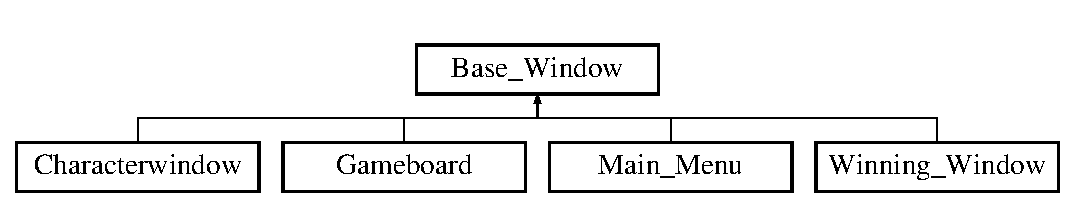
\includegraphics[height=2.000000cm]{classBase__Window}
\end{center}
\end{figure}
\subsection*{Public Member Functions}
\begin{DoxyCompactItemize}
\item 
\hyperlink{classBase__Window_a89fc36aacdebe0a28371648c16a51be6}{Base\+\_\+\+Window} ()=default
\begin{DoxyCompactList}\small\item\em A default constructor. \end{DoxyCompactList}\end{DoxyCompactItemize}
\subsection*{Protected Member Functions}
\begin{DoxyCompactItemize}
\item 
virtual void \hyperlink{classBase__Window_a0d0e107e9eb19bd74b25f4465688e862}{load\+\_\+textures} ()=0
\begin{DoxyCompactList}\small\item\em A pure virtual function loading textures needed for the window. \end{DoxyCompactList}\item 
sf\+::\+Texture \& \hyperlink{classBase__Window_a7795a731d3e0dba029219b0d81954dfc}{get\+\_\+texture} (std\+::string const \&filename)
\begin{DoxyCompactList}\small\item\em A function member returning a texture based on specified filename of texture. \end{DoxyCompactList}\end{DoxyCompactItemize}
\subsection*{Protected Attributes}
\begin{DoxyCompactItemize}
\item 
\mbox{\Hypertarget{classBase__Window_aaf143aef62737103510092d9eda06118}\label{classBase__Window_aaf143aef62737103510092d9eda06118}} 
sf\+::\+Sprite {\bfseries bg\+\_\+sprite}
\item 
\mbox{\Hypertarget{classBase__Window_a95819b9928fd4943c0478e2f9baa3842}\label{classBase__Window_a95819b9928fd4943c0478e2f9baa3842}} 
sf\+::\+Font {\bfseries font}
\item 
\mbox{\Hypertarget{classBase__Window_a0063751d92040019a7086dfc39808274}\label{classBase__Window_a0063751d92040019a7086dfc39808274}} 
std\+::map$<$ std\+::string, sf\+::\+Texture $>$ {\bfseries textures}
\end{DoxyCompactItemize}


\subsection{Detailed Description}
An abstract class representing a window. 

An abstract (pure virtual) class inheriting a \char`\"{}sf\+::\+Render\+Window\char`\"{} from the S\+F\+ML library to behave as a window. In addition the class also has other variable members every window wants to have in the game. 

\subsection{Constructor \& Destructor Documentation}
\mbox{\Hypertarget{classBase__Window_a89fc36aacdebe0a28371648c16a51be6}\label{classBase__Window_a89fc36aacdebe0a28371648c16a51be6}} 
\index{Base\+\_\+\+Window@{Base\+\_\+\+Window}!Base\+\_\+\+Window@{Base\+\_\+\+Window}}
\index{Base\+\_\+\+Window@{Base\+\_\+\+Window}!Base\+\_\+\+Window@{Base\+\_\+\+Window}}
\subsubsection{\texorpdfstring{Base\+\_\+\+Window()}{Base\_Window()}}
{\footnotesize\ttfamily Base\+\_\+\+Window\+::\+Base\+\_\+\+Window (\begin{DoxyParamCaption}{ }\end{DoxyParamCaption})\hspace{0.3cm}{\ttfamily [default]}}



A default constructor. 

Constructor uses compiler\textquotesingle{}s default way of constructing class. 

\subsection{Member Function Documentation}
\mbox{\Hypertarget{classBase__Window_a7795a731d3e0dba029219b0d81954dfc}\label{classBase__Window_a7795a731d3e0dba029219b0d81954dfc}} 
\index{Base\+\_\+\+Window@{Base\+\_\+\+Window}!get\+\_\+texture@{get\+\_\+texture}}
\index{get\+\_\+texture@{get\+\_\+texture}!Base\+\_\+\+Window@{Base\+\_\+\+Window}}
\subsubsection{\texorpdfstring{get\+\_\+texture()}{get\_texture()}}
{\footnotesize\ttfamily sf\+::\+Texture \& Base\+\_\+\+Window\+::get\+\_\+texture (\begin{DoxyParamCaption}\item[{std\+::string const \&}]{filename }\end{DoxyParamCaption})\hspace{0.3cm}{\ttfamily [protected]}}



A function member returning a texture based on specified filename of texture. 


\begin{DoxyParams}{Parameters}
{\em filename} & a std\+::string with the name of the texture file. \\
\hline
\end{DoxyParams}
\begin{DoxyReturn}{Returns}
The texture 
\end{DoxyReturn}
\mbox{\Hypertarget{classBase__Window_a0d0e107e9eb19bd74b25f4465688e862}\label{classBase__Window_a0d0e107e9eb19bd74b25f4465688e862}} 
\index{Base\+\_\+\+Window@{Base\+\_\+\+Window}!load\+\_\+textures@{load\+\_\+textures}}
\index{load\+\_\+textures@{load\+\_\+textures}!Base\+\_\+\+Window@{Base\+\_\+\+Window}}
\subsubsection{\texorpdfstring{load\+\_\+textures()}{load\_textures()}}
{\footnotesize\ttfamily virtual void Base\+\_\+\+Window\+::load\+\_\+textures (\begin{DoxyParamCaption}{ }\end{DoxyParamCaption})\hspace{0.3cm}{\ttfamily [protected]}, {\ttfamily [pure virtual]}}



A pure virtual function loading textures needed for the window. 

Loads all the textures needed for the window. This is done by creating a container in which the filename of the texture is connected to the texture object. Since all windows want to load textures in a different way the function needs to be overrided by each subwindow. 

The documentation for this class was generated from the following files\+:\begin{DoxyCompactItemize}
\item 
base\+\_\+window.\+h\item 
base\+\_\+window.\+cpp\end{DoxyCompactItemize}

\hypertarget{classCharacterwindow}{}\section{Characterwindow Class Reference}
\label{classCharacterwindow}\index{Characterwindow@{Characterwindow}}


A class representing a character selection window.  




{\ttfamily \#include $<$characterwindow.\+h$>$}

Inheritance diagram for Characterwindow\+:\begin{figure}[H]
\begin{center}
\leavevmode
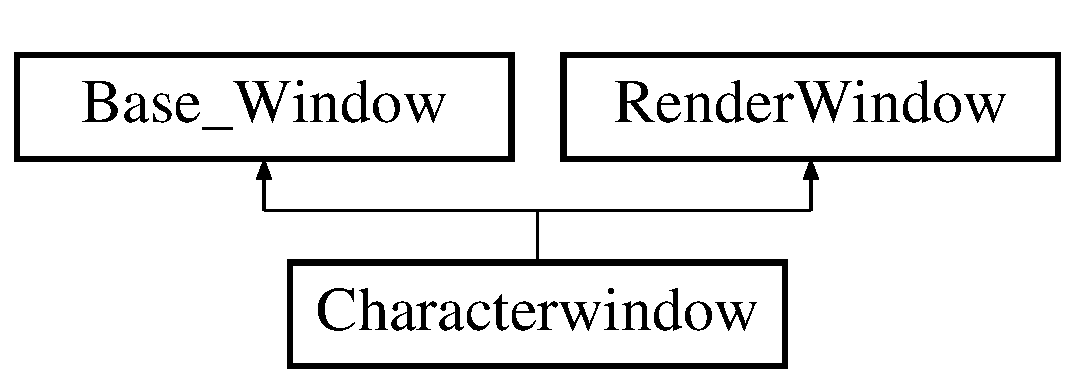
\includegraphics[height=2.000000cm]{classCharacterwindow}
\end{center}
\end{figure}
\subsection*{Public Member Functions}
\begin{DoxyCompactItemize}
\item 
\hyperlink{classCharacterwindow_a2f9d2f2231c33265918bc9697f03c894}{Characterwindow} ()=default
\begin{DoxyCompactList}\small\item\em A default constructor. \end{DoxyCompactList}\item 
void \hyperlink{classCharacterwindow_a0e7738c002afb23bb1d571d5d4f1dd1d}{initialize} ()
\begin{DoxyCompactList}\small\item\em Initialize the window. \end{DoxyCompactList}\item 
void \hyperlink{classCharacterwindow_aaca1dea6e04dbd2843907d652dcf2fb0}{update\+Graphics} ()
\begin{DoxyCompactList}\small\item\em Update graphical display of the window. \end{DoxyCompactList}\item 
void \hyperlink{classCharacterwindow_a3e74d9d40166eb88e2259f4f0d1da2ab}{change\+Character} (Direction direction, bool is\+\_\+player1=true)
\begin{DoxyCompactList}\small\item\em Change selected character for a player. \end{DoxyCompactList}\item 
unsigned int \hyperlink{classCharacterwindow_a9af7aeece3281823e2e972beb797283a}{get\+Selected\+Character\+Id} (bool is\+\_\+player1=true) const
\begin{DoxyCompactList}\small\item\em Get the id of the selected character. \end{DoxyCompactList}\end{DoxyCompactItemize}
\subsection*{Additional Inherited Members}


\subsection{Detailed Description}
A class representing a character selection window. 

A class inheriting from \char`\"{}\+Base\+\_\+\+Window\char`\"{} to make class represent a window. In addition the class contains members needed for a character selection window in the game. A character selection window is where the players select a character to play (and other possible options before a match starts). 

\subsection{Constructor \& Destructor Documentation}
\mbox{\Hypertarget{classCharacterwindow_a2f9d2f2231c33265918bc9697f03c894}\label{classCharacterwindow_a2f9d2f2231c33265918bc9697f03c894}} 
\index{Characterwindow@{Characterwindow}!Characterwindow@{Characterwindow}}
\index{Characterwindow@{Characterwindow}!Characterwindow@{Characterwindow}}
\subsubsection{\texorpdfstring{Characterwindow()}{Characterwindow()}}
{\footnotesize\ttfamily Characterwindow\+::\+Characterwindow (\begin{DoxyParamCaption}{ }\end{DoxyParamCaption})\hspace{0.3cm}{\ttfamily [default]}}



A default constructor. 

Constructor uses compiler\textquotesingle{}s default way of constructing class. 

\subsection{Member Function Documentation}
\mbox{\Hypertarget{classCharacterwindow_a3e74d9d40166eb88e2259f4f0d1da2ab}\label{classCharacterwindow_a3e74d9d40166eb88e2259f4f0d1da2ab}} 
\index{Characterwindow@{Characterwindow}!change\+Character@{change\+Character}}
\index{change\+Character@{change\+Character}!Characterwindow@{Characterwindow}}
\subsubsection{\texorpdfstring{change\+Character()}{changeCharacter()}}
{\footnotesize\ttfamily void Characterwindow\+::change\+Character (\begin{DoxyParamCaption}\item[{Direction}]{direction,  }\item[{bool}]{is\+\_\+player1 = {\ttfamily true} }\end{DoxyParamCaption})}



Change selected character for a player. 

Changes either player 1\textquotesingle{}s or player 2\textquotesingle{}s character by moving player in the desired direction in the character list. N\+O\+TE\+: It\textquotesingle{}s only moved if possible. 
\begin{DoxyParams}{Parameters}
{\em direction} & The direction to go in the character list \\
\hline
{\em is\+\_\+player1} & If player 1 should change character or not (player 2) (default is true) \\
\hline
\end{DoxyParams}
\mbox{\Hypertarget{classCharacterwindow_a9af7aeece3281823e2e972beb797283a}\label{classCharacterwindow_a9af7aeece3281823e2e972beb797283a}} 
\index{Characterwindow@{Characterwindow}!get\+Selected\+Character\+Id@{get\+Selected\+Character\+Id}}
\index{get\+Selected\+Character\+Id@{get\+Selected\+Character\+Id}!Characterwindow@{Characterwindow}}
\subsubsection{\texorpdfstring{get\+Selected\+Character\+Id()}{getSelectedCharacterId()}}
{\footnotesize\ttfamily unsigned int Characterwindow\+::get\+Selected\+Character\+Id (\begin{DoxyParamCaption}\item[{bool}]{is\+\_\+player1 = {\ttfamily true} }\end{DoxyParamCaption}) const}



Get the id of the selected character. 

Get the selected character id for the specified player. 
\begin{DoxyParams}{Parameters}
{\em is\+\_\+player1} & If you should return selected character id for player 1 or not (player 2) (default is player 1) \\
\hline
\end{DoxyParams}
\begin{DoxyReturn}{Returns}
Selected character id for the specified player 
\end{DoxyReturn}
\mbox{\Hypertarget{classCharacterwindow_a0e7738c002afb23bb1d571d5d4f1dd1d}\label{classCharacterwindow_a0e7738c002afb23bb1d571d5d4f1dd1d}} 
\index{Characterwindow@{Characterwindow}!initialize@{initialize}}
\index{initialize@{initialize}!Characterwindow@{Characterwindow}}
\subsubsection{\texorpdfstring{initialize()}{initialize()}}
{\footnotesize\ttfamily void Characterwindow\+::initialize (\begin{DoxyParamCaption}{ }\end{DoxyParamCaption})}



Initialize the window. 

Initializes member variables by for example setting textures, position and sizes. \mbox{\Hypertarget{classCharacterwindow_aaca1dea6e04dbd2843907d652dcf2fb0}\label{classCharacterwindow_aaca1dea6e04dbd2843907d652dcf2fb0}} 
\index{Characterwindow@{Characterwindow}!update\+Graphics@{update\+Graphics}}
\index{update\+Graphics@{update\+Graphics}!Characterwindow@{Characterwindow}}
\subsubsection{\texorpdfstring{update\+Graphics()}{updateGraphics()}}
{\footnotesize\ttfamily void Characterwindow\+::update\+Graphics (\begin{DoxyParamCaption}{ }\end{DoxyParamCaption})}



Update graphical display of the window. 

Member function to update the graphics of the window based on possible changes 

The documentation for this class was generated from the following files\+:\begin{DoxyCompactItemize}
\item 
characterwindow.\+h\item 
characterwindow.\+cpp\end{DoxyCompactItemize}

\hypertarget{classEntity}{}\section{Entity Class Reference}
\label{classEntity}\index{Entity@{Entity}}


A pure virtual class representing a movable entity.  




{\ttfamily \#include $<$entity.\+h$>$}

Inheritance diagram for Entity\+:\begin{figure}[H]
\begin{center}
\leavevmode
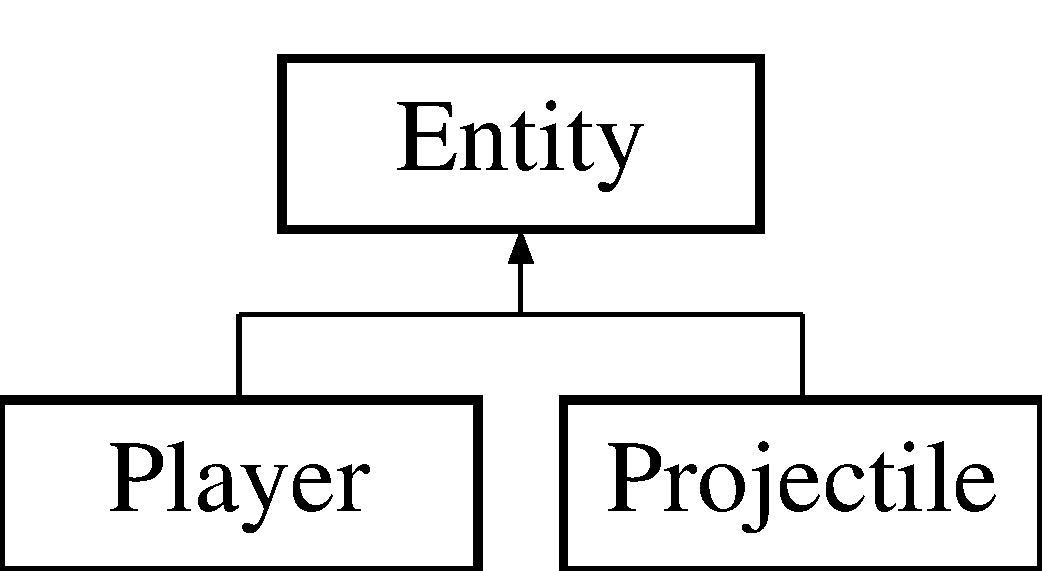
\includegraphics[height=2.000000cm]{classEntity}
\end{center}
\end{figure}
\subsection*{Public Member Functions}
\begin{DoxyCompactItemize}
\item 
void \hyperlink{classEntity_aba38705a06cf12c0e87b8b42713f3ce7}{move} (Direction direction, unsigned int steps=1)
\begin{DoxyCompactList}\small\item\em Moves the entity in a direction. \end{DoxyCompactList}\item 
void \hyperlink{classEntity_a8c7f316068b48003621f301b24d6ff47}{change\+Direction} (Direction direction)
\begin{DoxyCompactList}\small\item\em Change direction entity is faced. \end{DoxyCompactList}\item 
void \hyperlink{classEntity_abfef59d2e7f81727d43a86425e8e06df}{set\+Position} (\hyperlink{structPoint}{Point} pos)
\begin{DoxyCompactList}\small\item\em Change position of the entity. \end{DoxyCompactList}\item 
void \hyperlink{classEntity_a8871ade33babf42d554f498154f35e26}{set\+Position} (int x, int y)
\begin{DoxyCompactList}\small\item\em Change position of the entity. \end{DoxyCompactList}\item 
\hyperlink{structPoint}{Point} \hyperlink{classEntity_a0db2ab8dd08e0da409133786803bd4e0}{get\+Position} () const
\begin{DoxyCompactList}\small\item\em Get the position of the entity. \end{DoxyCompactList}\item 
std\+::string \hyperlink{classEntity_a403f69eb888da7c5a690b79c658cdf47}{get\+Name} () const
\begin{DoxyCompactList}\small\item\em Get the name of the entity. \end{DoxyCompactList}\item 
double \hyperlink{classEntity_a7cf65c6f73d2a17e59a26344c8ffb999}{get\+Speed} () const
\begin{DoxyCompactList}\small\item\em Get the speed of the entity. \end{DoxyCompactList}\item 
unsigned int \hyperlink{classEntity_a002be2c6f13d59bff1806ef8815478d5}{get\+Width} () const
\begin{DoxyCompactList}\small\item\em Get the width of the entity. \end{DoxyCompactList}\item 
unsigned int \hyperlink{classEntity_a5bbd1da83a9212d0de7e6d0dca659bf8}{get\+Height} () const
\begin{DoxyCompactList}\small\item\em Get the height of the entity. \end{DoxyCompactList}\item 
std\+::string \hyperlink{classEntity_a0d10637b4a1e31e139fcf992227d4ef8}{get\+Sprite\+Source} () const
\begin{DoxyCompactList}\small\item\em Get the source to the sprite image. \end{DoxyCompactList}\item 
Direction \hyperlink{classEntity_a6e758491533926eb0c27d4ddad83a210}{get\+Direction} () const
\begin{DoxyCompactList}\small\item\em Get the direction the entity is currently facing. \end{DoxyCompactList}\end{DoxyCompactItemize}
\subsection*{Protected Member Functions}
\begin{DoxyCompactItemize}
\item 
virtual bool \hyperlink{classEntity_a6a8f776c063333b5756e720d9b6dfeac}{can\+\_\+move} (Direction direction) const =0
\begin{DoxyCompactList}\small\item\em A pure virtual function that checks if the entity can move or not. \end{DoxyCompactList}\end{DoxyCompactItemize}
\subsection*{Protected Attributes}
\begin{DoxyCompactItemize}
\item 
\mbox{\Hypertarget{classEntity_a931b21fbdebb1a5963b4bcab5df128f5}\label{classEntity_a931b21fbdebb1a5963b4bcab5df128f5}} 
std\+::string {\bfseries name}
\item 
\mbox{\Hypertarget{classEntity_a0fa3249cb9d74341cbd1343ef735e741}\label{classEntity_a0fa3249cb9d74341cbd1343ef735e741}} 
\hyperlink{structPoint}{Point} {\bfseries position}
\item 
\mbox{\Hypertarget{classEntity_a1376f94e972719f8153716ccfda85c6f}\label{classEntity_a1376f94e972719f8153716ccfda85c6f}} 
Direction {\bfseries dir}
\item 
\mbox{\Hypertarget{classEntity_a98572d956beb757675259e55bf79d5fd}\label{classEntity_a98572d956beb757675259e55bf79d5fd}} 
double {\bfseries speed}
\item 
\mbox{\Hypertarget{classEntity_ac5e09232fb967bf716cc6e6684d32cea}\label{classEntity_ac5e09232fb967bf716cc6e6684d32cea}} 
unsigned int {\bfseries width}
\item 
\mbox{\Hypertarget{classEntity_aebf02bb745e69e68f44d5b5cee318d97}\label{classEntity_aebf02bb745e69e68f44d5b5cee318d97}} 
unsigned int {\bfseries height}
\item 
\mbox{\Hypertarget{classEntity_a998573f778e41028ebae46d195314ab9}\label{classEntity_a998573f778e41028ebae46d195314ab9}} 
std\+::string {\bfseries sprite\+\_\+src}
\end{DoxyCompactItemize}


\subsection{Detailed Description}
A pure virtual class representing a movable entity. 

The class has basic members all movable entities should have, such as position, direction, size etc. 

\subsection{Member Function Documentation}
\mbox{\Hypertarget{classEntity_a6a8f776c063333b5756e720d9b6dfeac}\label{classEntity_a6a8f776c063333b5756e720d9b6dfeac}} 
\index{Entity@{Entity}!can\+\_\+move@{can\+\_\+move}}
\index{can\+\_\+move@{can\+\_\+move}!Entity@{Entity}}
\subsubsection{\texorpdfstring{can\+\_\+move()}{can\_move()}}
{\footnotesize\ttfamily virtual bool Entity\+::can\+\_\+move (\begin{DoxyParamCaption}\item[{Direction}]{direction }\end{DoxyParamCaption}) const\hspace{0.3cm}{\ttfamily [protected]}, {\ttfamily [pure virtual]}}



A pure virtual function that checks if the entity can move or not. 

Checks if the entity can move or not. Since this is checked differently for each entity type the function is pure virtual. 
\begin{DoxyParams}{Parameters}
{\em direction} & \\
\hline
\end{DoxyParams}
\begin{DoxyReturn}{Returns}
If entity can move or not 
\end{DoxyReturn}
\mbox{\Hypertarget{classEntity_a8c7f316068b48003621f301b24d6ff47}\label{classEntity_a8c7f316068b48003621f301b24d6ff47}} 
\index{Entity@{Entity}!change\+Direction@{change\+Direction}}
\index{change\+Direction@{change\+Direction}!Entity@{Entity}}
\subsubsection{\texorpdfstring{change\+Direction()}{changeDirection()}}
{\footnotesize\ttfamily void Entity\+::change\+Direction (\begin{DoxyParamCaption}\item[{Direction}]{direction }\end{DoxyParamCaption})}



Change direction entity is faced. 


\begin{DoxyParams}{Parameters}
{\em direction} & Direction to change into \\
\hline
\end{DoxyParams}
\mbox{\Hypertarget{classEntity_a6e758491533926eb0c27d4ddad83a210}\label{classEntity_a6e758491533926eb0c27d4ddad83a210}} 
\index{Entity@{Entity}!get\+Direction@{get\+Direction}}
\index{get\+Direction@{get\+Direction}!Entity@{Entity}}
\subsubsection{\texorpdfstring{get\+Direction()}{getDirection()}}
{\footnotesize\ttfamily Direction Entity\+::get\+Direction (\begin{DoxyParamCaption}{ }\end{DoxyParamCaption}) const}



Get the direction the entity is currently facing. 

\begin{DoxyReturn}{Returns}
Direction entity is currently facing 
\end{DoxyReturn}
\mbox{\Hypertarget{classEntity_a5bbd1da83a9212d0de7e6d0dca659bf8}\label{classEntity_a5bbd1da83a9212d0de7e6d0dca659bf8}} 
\index{Entity@{Entity}!get\+Height@{get\+Height}}
\index{get\+Height@{get\+Height}!Entity@{Entity}}
\subsubsection{\texorpdfstring{get\+Height()}{getHeight()}}
{\footnotesize\ttfamily unsigned int Entity\+::get\+Height (\begin{DoxyParamCaption}{ }\end{DoxyParamCaption}) const}



Get the height of the entity. 

\begin{DoxyReturn}{Returns}
Height of the entity 
\end{DoxyReturn}
\mbox{\Hypertarget{classEntity_a403f69eb888da7c5a690b79c658cdf47}\label{classEntity_a403f69eb888da7c5a690b79c658cdf47}} 
\index{Entity@{Entity}!get\+Name@{get\+Name}}
\index{get\+Name@{get\+Name}!Entity@{Entity}}
\subsubsection{\texorpdfstring{get\+Name()}{getName()}}
{\footnotesize\ttfamily std\+::string Entity\+::get\+Name (\begin{DoxyParamCaption}{ }\end{DoxyParamCaption}) const}



Get the name of the entity. 

\begin{DoxyReturn}{Returns}
Name of entity 
\end{DoxyReturn}
\mbox{\Hypertarget{classEntity_a0db2ab8dd08e0da409133786803bd4e0}\label{classEntity_a0db2ab8dd08e0da409133786803bd4e0}} 
\index{Entity@{Entity}!get\+Position@{get\+Position}}
\index{get\+Position@{get\+Position}!Entity@{Entity}}
\subsubsection{\texorpdfstring{get\+Position()}{getPosition()}}
{\footnotesize\ttfamily \hyperlink{structPoint}{Point} Entity\+::get\+Position (\begin{DoxyParamCaption}{ }\end{DoxyParamCaption}) const}



Get the position of the entity. 

\begin{DoxyReturn}{Returns}
Position of entity 
\end{DoxyReturn}
\mbox{\Hypertarget{classEntity_a7cf65c6f73d2a17e59a26344c8ffb999}\label{classEntity_a7cf65c6f73d2a17e59a26344c8ffb999}} 
\index{Entity@{Entity}!get\+Speed@{get\+Speed}}
\index{get\+Speed@{get\+Speed}!Entity@{Entity}}
\subsubsection{\texorpdfstring{get\+Speed()}{getSpeed()}}
{\footnotesize\ttfamily double Entity\+::get\+Speed (\begin{DoxyParamCaption}{ }\end{DoxyParamCaption}) const}



Get the speed of the entity. 

\begin{DoxyReturn}{Returns}
Speed of entity 
\end{DoxyReturn}
\mbox{\Hypertarget{classEntity_a0d10637b4a1e31e139fcf992227d4ef8}\label{classEntity_a0d10637b4a1e31e139fcf992227d4ef8}} 
\index{Entity@{Entity}!get\+Sprite\+Source@{get\+Sprite\+Source}}
\index{get\+Sprite\+Source@{get\+Sprite\+Source}!Entity@{Entity}}
\subsubsection{\texorpdfstring{get\+Sprite\+Source()}{getSpriteSource()}}
{\footnotesize\ttfamily std\+::string Entity\+::get\+Sprite\+Source (\begin{DoxyParamCaption}{ }\end{DoxyParamCaption}) const}



Get the source to the sprite image. 

\begin{DoxyReturn}{Returns}
Source to the sprite image 
\end{DoxyReturn}
\mbox{\Hypertarget{classEntity_a002be2c6f13d59bff1806ef8815478d5}\label{classEntity_a002be2c6f13d59bff1806ef8815478d5}} 
\index{Entity@{Entity}!get\+Width@{get\+Width}}
\index{get\+Width@{get\+Width}!Entity@{Entity}}
\subsubsection{\texorpdfstring{get\+Width()}{getWidth()}}
{\footnotesize\ttfamily unsigned int Entity\+::get\+Width (\begin{DoxyParamCaption}{ }\end{DoxyParamCaption}) const}



Get the width of the entity. 

\begin{DoxyReturn}{Returns}
Width of entity 
\end{DoxyReturn}
\mbox{\Hypertarget{classEntity_aba38705a06cf12c0e87b8b42713f3ce7}\label{classEntity_aba38705a06cf12c0e87b8b42713f3ce7}} 
\index{Entity@{Entity}!move@{move}}
\index{move@{move}!Entity@{Entity}}
\subsubsection{\texorpdfstring{move()}{move()}}
{\footnotesize\ttfamily void Entity\+::move (\begin{DoxyParamCaption}\item[{Direction}]{direction,  }\item[{unsigned int}]{steps = {\ttfamily 1} }\end{DoxyParamCaption})}



Moves the entity in a direction. 

Moves the entity in the specified direction a specified amount of steps (essentially the same as distance) 
\begin{DoxyParams}{Parameters}
{\em direction} & The direction to move in \\
\hline
{\em steps} & Amount of steps to move entity (essentially the same as distance) \\
\hline
\end{DoxyParams}
\mbox{\Hypertarget{classEntity_abfef59d2e7f81727d43a86425e8e06df}\label{classEntity_abfef59d2e7f81727d43a86425e8e06df}} 
\index{Entity@{Entity}!set\+Position@{set\+Position}}
\index{set\+Position@{set\+Position}!Entity@{Entity}}
\subsubsection{\texorpdfstring{set\+Position()}{setPosition()}\hspace{0.1cm}{\footnotesize\ttfamily [1/2]}}
{\footnotesize\ttfamily void Entity\+::set\+Position (\begin{DoxyParamCaption}\item[{\hyperlink{structPoint}{Point}}]{pos }\end{DoxyParamCaption})}



Change position of the entity. 


\begin{DoxyParams}{Parameters}
{\em pos} & Specified position \\
\hline
\end{DoxyParams}
\mbox{\Hypertarget{classEntity_a8871ade33babf42d554f498154f35e26}\label{classEntity_a8871ade33babf42d554f498154f35e26}} 
\index{Entity@{Entity}!set\+Position@{set\+Position}}
\index{set\+Position@{set\+Position}!Entity@{Entity}}
\subsubsection{\texorpdfstring{set\+Position()}{setPosition()}\hspace{0.1cm}{\footnotesize\ttfamily [2/2]}}
{\footnotesize\ttfamily void Entity\+::set\+Position (\begin{DoxyParamCaption}\item[{int}]{x,  }\item[{int}]{y }\end{DoxyParamCaption})}



Change position of the entity. 


\begin{DoxyParams}{Parameters}
{\em x} & x-\/position \\
\hline
{\em y} & y-\/position \\
\hline
\end{DoxyParams}


The documentation for this class was generated from the following files\+:\begin{DoxyCompactItemize}
\item 
entity.\+h\item 
entity.\+cpp\end{DoxyCompactItemize}

\hypertarget{classGame38}{}\section{Game38 Class Reference}
\label{classGame38}\index{Game38@{Game38}}


A class for running the game \char`\"{}game38\char`\"{}.  




{\ttfamily \#include $<$game38.\+h$>$}

\subsection*{Public Member Functions}
\begin{DoxyCompactItemize}
\item 
\hyperlink{classGame38_a6279a9c93ae21dead3ee6165c1afe04c}{Game38} ()=default
\begin{DoxyCompactList}\small\item\em A default constructor. \end{DoxyCompactList}\item 
void \hyperlink{classGame38_ab9e0b292923fbef270ab0cea6c59cf23}{run} ()
\begin{DoxyCompactList}\small\item\em Run the game. \end{DoxyCompactList}\end{DoxyCompactItemize}


\subsection{Detailed Description}
A class for running the game \char`\"{}game38\char`\"{}. 

A class representing a playable \char`\"{}game38\char`\"{}. The only thing needed to play is to call function \char`\"{}run()\char`\"{}. 

\subsection{Constructor \& Destructor Documentation}
\mbox{\Hypertarget{classGame38_a6279a9c93ae21dead3ee6165c1afe04c}\label{classGame38_a6279a9c93ae21dead3ee6165c1afe04c}} 
\index{Game38@{Game38}!Game38@{Game38}}
\index{Game38@{Game38}!Game38@{Game38}}
\subsubsection{\texorpdfstring{Game38()}{Game38()}}
{\footnotesize\ttfamily Game38\+::\+Game38 (\begin{DoxyParamCaption}{ }\end{DoxyParamCaption})\hspace{0.3cm}{\ttfamily [default]}}



A default constructor. 

Constructor uses compiler\textquotesingle{}s default way of constructing class. 

\subsection{Member Function Documentation}
\mbox{\Hypertarget{classGame38_ab9e0b292923fbef270ab0cea6c59cf23}\label{classGame38_ab9e0b292923fbef270ab0cea6c59cf23}} 
\index{Game38@{Game38}!run@{run}}
\index{run@{run}!Game38@{Game38}}
\subsubsection{\texorpdfstring{run()}{run()}}
{\footnotesize\ttfamily void Game38\+::run (\begin{DoxyParamCaption}{ }\end{DoxyParamCaption})}



Run the game. 

Start and run the game while something doesn\textquotesingle{}t tell the game to quit. 

The documentation for this class was generated from the following files\+:\begin{DoxyCompactItemize}
\item 
game38.\+h\item 
game38.\+cpp\end{DoxyCompactItemize}

\hypertarget{classGameboard}{}\section{Gameboard Class Reference}
\label{classGameboard}\index{Gameboard@{Gameboard}}


A class representing a main menu window.  




{\ttfamily \#include $<$gameboard.\+h$>$}

Inheritance diagram for Gameboard\+:\begin{figure}[H]
\begin{center}
\leavevmode
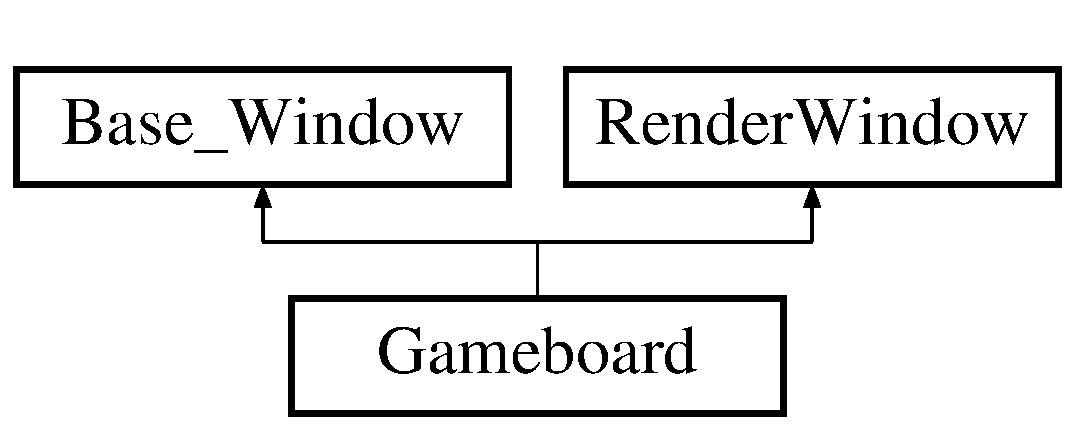
\includegraphics[height=2.000000cm]{classGameboard}
\end{center}
\end{figure}
\subsection*{Public Member Functions}
\begin{DoxyCompactItemize}
\item 
\hyperlink{classGameboard_a35e7c6d4e378d0e62a5cd964933410cf}{Gameboard} ()=default
\begin{DoxyCompactList}\small\item\em A default constructor. \end{DoxyCompactList}\item 
void \hyperlink{classGameboard_a26dc97929c4382659d1f52bb0f8bb19a}{initialize} (\hyperlink{classLevel}{Level} const \&level, \hyperlink{classPlayer}{Player} const \&player1, \hyperlink{classPlayer}{Player} const \&player2)
\begin{DoxyCompactList}\small\item\em Initializes member variables of the gameboard window. \end{DoxyCompactList}\item 
void \hyperlink{classGameboard_a6192fda60355f9bb0175af2fc50f40d0}{update\+Graphics} (\hyperlink{classLevel}{Level} const \&level, \hyperlink{classPlayer}{Player} const \&player1, \hyperlink{classPlayer}{Player} const \&player2)
\begin{DoxyCompactList}\small\item\em Update graphical display of the gameboard window. \end{DoxyCompactList}\end{DoxyCompactItemize}
\subsection*{Additional Inherited Members}


\subsection{Detailed Description}
A class representing a main menu window. 

A class inheriting from \char`\"{}\+Base\+\_\+\+Window\char`\"{} to make class represent a window. In addition the class contains members needed for a gameboard in the game. A gameboard is a graphical representation of a level with two players fighting. 

\subsection{Constructor \& Destructor Documentation}
\mbox{\Hypertarget{classGameboard_a35e7c6d4e378d0e62a5cd964933410cf}\label{classGameboard_a35e7c6d4e378d0e62a5cd964933410cf}} 
\index{Gameboard@{Gameboard}!Gameboard@{Gameboard}}
\index{Gameboard@{Gameboard}!Gameboard@{Gameboard}}
\subsubsection{\texorpdfstring{Gameboard()}{Gameboard()}}
{\footnotesize\ttfamily Gameboard\+::\+Gameboard (\begin{DoxyParamCaption}{ }\end{DoxyParamCaption})\hspace{0.3cm}{\ttfamily [default]}}



A default constructor. 

Constructor uses compiler\textquotesingle{}s default way of constructing class. 

\subsection{Member Function Documentation}
\mbox{\Hypertarget{classGameboard_a26dc97929c4382659d1f52bb0f8bb19a}\label{classGameboard_a26dc97929c4382659d1f52bb0f8bb19a}} 
\index{Gameboard@{Gameboard}!initialize@{initialize}}
\index{initialize@{initialize}!Gameboard@{Gameboard}}
\subsubsection{\texorpdfstring{initialize()}{initialize()}}
{\footnotesize\ttfamily void Gameboard\+::initialize (\begin{DoxyParamCaption}\item[{\hyperlink{classLevel}{Level} const \&}]{level,  }\item[{\hyperlink{classPlayer}{Player} const \&}]{player1,  }\item[{\hyperlink{classPlayer}{Player} const \&}]{player2 }\end{DoxyParamCaption})}



Initializes member variables of the gameboard window. 

Initializes member variables based on the specified level, player 1 and player 2 
\begin{DoxyParams}{Parameters}
{\em level} & The specified level for gameboard to represent \\
\hline
{\em player1} & \hyperlink{classPlayer}{Player} 1 on the gameboard \\
\hline
{\em player2} & \hyperlink{classPlayer}{Player} 2 on the gameboard \\
\hline
\end{DoxyParams}
\mbox{\Hypertarget{classGameboard_a6192fda60355f9bb0175af2fc50f40d0}\label{classGameboard_a6192fda60355f9bb0175af2fc50f40d0}} 
\index{Gameboard@{Gameboard}!update\+Graphics@{update\+Graphics}}
\index{update\+Graphics@{update\+Graphics}!Gameboard@{Gameboard}}
\subsubsection{\texorpdfstring{update\+Graphics()}{updateGraphics()}}
{\footnotesize\ttfamily void Gameboard\+::update\+Graphics (\begin{DoxyParamCaption}\item[{\hyperlink{classLevel}{Level} const \&}]{level,  }\item[{\hyperlink{classPlayer}{Player} const \&}]{player1,  }\item[{\hyperlink{classPlayer}{Player} const \&}]{player2 }\end{DoxyParamCaption})}



Update graphical display of the gameboard window. 

Updates graphics of window based on possible changes, the specified level, player 1 and player 2 
\begin{DoxyParams}{Parameters}
{\em level} & The specified level for gameboard to represent \\
\hline
{\em player1} & \hyperlink{classPlayer}{Player} 1 on the gameboard \\
\hline
{\em player2} & \hyperlink{classPlayer}{Player} 2 on the gameboard \\
\hline
\end{DoxyParams}


The documentation for this class was generated from the following files\+:\begin{DoxyCompactItemize}
\item 
gameboard.\+h\item 
gameboard.\+cpp\end{DoxyCompactItemize}

\hypertarget{classLevel}{}\section{Level Class Reference}
\label{classLevel}\index{Level@{Level}}


A class representing a level where entity can move.  




{\ttfamily \#include $<$level.\+h$>$}

\subsection*{Public Member Functions}
\begin{DoxyCompactItemize}
\item 
\hyperlink{classLevel_ac1c79fc13a67584d22e3d7295cd3cc9d}{Level} ()=default
\begin{DoxyCompactList}\small\item\em A default constructor. \end{DoxyCompactList}\item 
\hyperlink{classLevel_a8fc569ff48384440a513dfc188d4f96d}{Level} (unsigned int level\+\_\+id)
\begin{DoxyCompactList}\small\item\em Constructs a level based on level id. \end{DoxyCompactList}\item 
void \hyperlink{classLevel_a403167dadfaccc9f5d9269845bcda34f}{add\+Player} (\hyperlink{classPlayer}{Player} \&player)
\begin{DoxyCompactList}\small\item\em Add a player to the level. \end{DoxyCompactList}\item 
void \hyperlink{classLevel_a9a1fb164259e6a8c91410ed992a8b878}{reload} ()
\begin{DoxyCompactList}\small\item\em Reload the level. \end{DoxyCompactList}\item 
std\+::string \hyperlink{classLevel_a0b6dd5b18919a849c374b67625a849fb}{get\+Name} () const
\begin{DoxyCompactList}\small\item\em Get name of the level. \end{DoxyCompactList}\item 
unsigned int \hyperlink{classLevel_ab37b554aa2379fb9c99fa4c83eef1823}{get\+Width} () const
\begin{DoxyCompactList}\small\item\em Get the width of the level. \end{DoxyCompactList}\item 
unsigned int \hyperlink{classLevel_a134002eee88eb3af6955241948309934}{get\+Height} () const
\begin{DoxyCompactList}\small\item\em Get the height of the level. \end{DoxyCompactList}\item 
std\+::string \hyperlink{classLevel_af7eb4bcc3f48dce1da830b4601cc8bb5}{get\+Bg\+Source} () const
\begin{DoxyCompactList}\small\item\em Get source to the background image of level. \end{DoxyCompactList}\end{DoxyCompactItemize}


\subsection{Detailed Description}
A class representing a level where entity can move. 

Essentially represents a gamebaord where entity can move. A level for example has a size and contains players and the player\textquotesingle{}s side of the board 

\subsection{Constructor \& Destructor Documentation}
\mbox{\Hypertarget{classLevel_ac1c79fc13a67584d22e3d7295cd3cc9d}\label{classLevel_ac1c79fc13a67584d22e3d7295cd3cc9d}} 
\index{Level@{Level}!Level@{Level}}
\index{Level@{Level}!Level@{Level}}
\subsubsection{\texorpdfstring{Level()}{Level()}\hspace{0.1cm}{\footnotesize\ttfamily [1/2]}}
{\footnotesize\ttfamily Level\+::\+Level (\begin{DoxyParamCaption}{ }\end{DoxyParamCaption})\hspace{0.3cm}{\ttfamily [default]}}



A default constructor. 

Constructor uses compiler\textquotesingle{}s default way of constructing class. \mbox{\Hypertarget{classLevel_a8fc569ff48384440a513dfc188d4f96d}\label{classLevel_a8fc569ff48384440a513dfc188d4f96d}} 
\index{Level@{Level}!Level@{Level}}
\index{Level@{Level}!Level@{Level}}
\subsubsection{\texorpdfstring{Level()}{Level()}\hspace{0.1cm}{\footnotesize\ttfamily [2/2]}}
{\footnotesize\ttfamily Level\+::\+Level (\begin{DoxyParamCaption}\item[{unsigned int}]{level\+\_\+id }\end{DoxyParamCaption})}



Constructs a level based on level id. 

Constructing a level with properties based on the level id 
\begin{DoxyParams}{Parameters}
{\em projectile\+\_\+id} & The specified level id \\
\hline
\end{DoxyParams}


\subsection{Member Function Documentation}
\mbox{\Hypertarget{classLevel_a403167dadfaccc9f5d9269845bcda34f}\label{classLevel_a403167dadfaccc9f5d9269845bcda34f}} 
\index{Level@{Level}!add\+Player@{add\+Player}}
\index{add\+Player@{add\+Player}!Level@{Level}}
\subsubsection{\texorpdfstring{add\+Player()}{addPlayer()}}
{\footnotesize\ttfamily void Level\+::add\+Player (\begin{DoxyParamCaption}\item[{\hyperlink{classPlayer}{Player} \&}]{player }\end{DoxyParamCaption})}



Add a player to the level. 

Adds a player to the level by pointing to the specified player 
\begin{DoxyParams}{Parameters}
{\em player} & A reference to the player \\
\hline
\end{DoxyParams}
\mbox{\Hypertarget{classLevel_af7eb4bcc3f48dce1da830b4601cc8bb5}\label{classLevel_af7eb4bcc3f48dce1da830b4601cc8bb5}} 
\index{Level@{Level}!get\+Bg\+Source@{get\+Bg\+Source}}
\index{get\+Bg\+Source@{get\+Bg\+Source}!Level@{Level}}
\subsubsection{\texorpdfstring{get\+Bg\+Source()}{getBgSource()}}
{\footnotesize\ttfamily std\+::string Level\+::get\+Bg\+Source (\begin{DoxyParamCaption}{ }\end{DoxyParamCaption}) const}



Get source to the background image of level. 

\begin{DoxyReturn}{Returns}
The source to the background image of level 
\end{DoxyReturn}
\mbox{\Hypertarget{classLevel_a134002eee88eb3af6955241948309934}\label{classLevel_a134002eee88eb3af6955241948309934}} 
\index{Level@{Level}!get\+Height@{get\+Height}}
\index{get\+Height@{get\+Height}!Level@{Level}}
\subsubsection{\texorpdfstring{get\+Height()}{getHeight()}}
{\footnotesize\ttfamily unsigned int Level\+::get\+Height (\begin{DoxyParamCaption}{ }\end{DoxyParamCaption}) const}



Get the height of the level. 

\begin{DoxyReturn}{Returns}
The height of the level 
\end{DoxyReturn}
\mbox{\Hypertarget{classLevel_a0b6dd5b18919a849c374b67625a849fb}\label{classLevel_a0b6dd5b18919a849c374b67625a849fb}} 
\index{Level@{Level}!get\+Name@{get\+Name}}
\index{get\+Name@{get\+Name}!Level@{Level}}
\subsubsection{\texorpdfstring{get\+Name()}{getName()}}
{\footnotesize\ttfamily std\+::string Level\+::get\+Name (\begin{DoxyParamCaption}{ }\end{DoxyParamCaption}) const}



Get name of the level. 

\begin{DoxyReturn}{Returns}
The name of the level 
\end{DoxyReturn}
\mbox{\Hypertarget{classLevel_ab37b554aa2379fb9c99fa4c83eef1823}\label{classLevel_ab37b554aa2379fb9c99fa4c83eef1823}} 
\index{Level@{Level}!get\+Width@{get\+Width}}
\index{get\+Width@{get\+Width}!Level@{Level}}
\subsubsection{\texorpdfstring{get\+Width()}{getWidth()}}
{\footnotesize\ttfamily unsigned int Level\+::get\+Width (\begin{DoxyParamCaption}{ }\end{DoxyParamCaption}) const}



Get the width of the level. 

\begin{DoxyReturn}{Returns}
The width of the level 
\end{DoxyReturn}
\mbox{\Hypertarget{classLevel_a9a1fb164259e6a8c91410ed992a8b878}\label{classLevel_a9a1fb164259e6a8c91410ed992a8b878}} 
\index{Level@{Level}!reload@{reload}}
\index{reload@{reload}!Level@{Level}}
\subsubsection{\texorpdfstring{reload()}{reload()}}
{\footnotesize\ttfamily void Level\+::reload (\begin{DoxyParamCaption}{ }\end{DoxyParamCaption})}



Reload the level. 

Reload the level by resetting players 

The documentation for this class was generated from the following files\+:\begin{DoxyCompactItemize}
\item 
level.\+h\item 
level.\+cpp\end{DoxyCompactItemize}

\hypertarget{classMain__Menu}{}\section{Main\+\_\+\+Menu Class Reference}
\label{classMain__Menu}\index{Main\+\_\+\+Menu@{Main\+\_\+\+Menu}}


A class representing a main menu window.  




{\ttfamily \#include $<$main\+\_\+menu.\+h$>$}

Inheritance diagram for Main\+\_\+\+Menu\+:\begin{figure}[H]
\begin{center}
\leavevmode
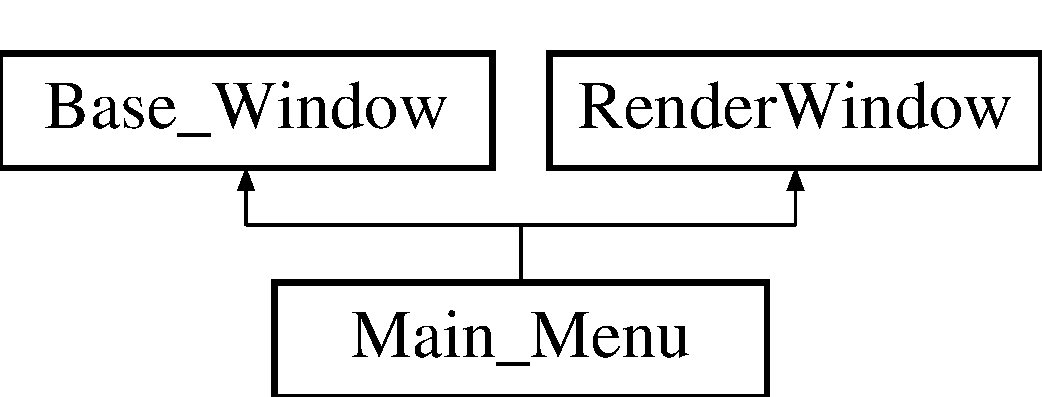
\includegraphics[height=2.000000cm]{classMain__Menu}
\end{center}
\end{figure}
\subsection*{Public Member Functions}
\begin{DoxyCompactItemize}
\item 
\hyperlink{classMain__Menu_a1f1fce181168ba08a7c2debe7e5333ef}{Main\+\_\+\+Menu} ()=default
\begin{DoxyCompactList}\small\item\em A default constructor. \end{DoxyCompactList}\item 
void \hyperlink{classMain__Menu_a453355fbb089549540a20eb7e540f04e}{initialize} ()
\begin{DoxyCompactList}\small\item\em Initializes member variables of the gameboard window. \end{DoxyCompactList}\item 
void \hyperlink{classMain__Menu_aa12d253d587d418b84550fffbc077478}{update\+Graphics} ()
\begin{DoxyCompactList}\small\item\em Update graphical display of the window. \end{DoxyCompactList}\item 
void \hyperlink{classMain__Menu_abd0bafbcc3a3aac9811cc6fde075b29c}{go\+Up} ()
\begin{DoxyCompactList}\small\item\em Go up in the menu. \end{DoxyCompactList}\item 
void \hyperlink{classMain__Menu_a0f95b5c387bd1cc18ba236a99060737c}{go\+Down} ()
\begin{DoxyCompactList}\small\item\em Go down in the menu. \end{DoxyCompactList}\item 
Menu\+\_\+\+Choice \hyperlink{classMain__Menu_a33b9a75fcda233154f81ed32f8f724d9}{get\+Menu\+Choice} ()
\begin{DoxyCompactList}\small\item\em Get user\textquotesingle{}s currently selected choice. \end{DoxyCompactList}\end{DoxyCompactItemize}
\subsection*{Additional Inherited Members}


\subsection{Detailed Description}
A class representing a main menu window. 

A class inheriting from \char`\"{}\+Base\+\_\+\+Window\char`\"{} to make class represent a window. In addition the class contains members needed for a main menu in the game. A main menu is where a user selects what to do in the game 

\subsection{Constructor \& Destructor Documentation}
\mbox{\Hypertarget{classMain__Menu_a1f1fce181168ba08a7c2debe7e5333ef}\label{classMain__Menu_a1f1fce181168ba08a7c2debe7e5333ef}} 
\index{Main\+\_\+\+Menu@{Main\+\_\+\+Menu}!Main\+\_\+\+Menu@{Main\+\_\+\+Menu}}
\index{Main\+\_\+\+Menu@{Main\+\_\+\+Menu}!Main\+\_\+\+Menu@{Main\+\_\+\+Menu}}
\subsubsection{\texorpdfstring{Main\+\_\+\+Menu()}{Main\_Menu()}}
{\footnotesize\ttfamily Main\+\_\+\+Menu\+::\+Main\+\_\+\+Menu (\begin{DoxyParamCaption}{ }\end{DoxyParamCaption})\hspace{0.3cm}{\ttfamily [default]}}



A default constructor. 

Constructor uses compiler\textquotesingle{}s default way of constructing class. 

\subsection{Member Function Documentation}
\mbox{\Hypertarget{classMain__Menu_a33b9a75fcda233154f81ed32f8f724d9}\label{classMain__Menu_a33b9a75fcda233154f81ed32f8f724d9}} 
\index{Main\+\_\+\+Menu@{Main\+\_\+\+Menu}!get\+Menu\+Choice@{get\+Menu\+Choice}}
\index{get\+Menu\+Choice@{get\+Menu\+Choice}!Main\+\_\+\+Menu@{Main\+\_\+\+Menu}}
\subsubsection{\texorpdfstring{get\+Menu\+Choice()}{getMenuChoice()}}
{\footnotesize\ttfamily Menu\+\_\+\+Choice Main\+\_\+\+Menu\+::get\+Menu\+Choice (\begin{DoxyParamCaption}{ }\end{DoxyParamCaption})}



Get user\textquotesingle{}s currently selected choice. 

\begin{DoxyReturn}{Returns}
The selected menu choice 
\end{DoxyReturn}
\mbox{\Hypertarget{classMain__Menu_a0f95b5c387bd1cc18ba236a99060737c}\label{classMain__Menu_a0f95b5c387bd1cc18ba236a99060737c}} 
\index{Main\+\_\+\+Menu@{Main\+\_\+\+Menu}!go\+Down@{go\+Down}}
\index{go\+Down@{go\+Down}!Main\+\_\+\+Menu@{Main\+\_\+\+Menu}}
\subsubsection{\texorpdfstring{go\+Down()}{goDown()}}
{\footnotesize\ttfamily void Main\+\_\+\+Menu\+::go\+Down (\begin{DoxyParamCaption}{ }\end{DoxyParamCaption})}



Go down in the menu. 

Go down in the menu by increasing selected index \mbox{\Hypertarget{classMain__Menu_abd0bafbcc3a3aac9811cc6fde075b29c}\label{classMain__Menu_abd0bafbcc3a3aac9811cc6fde075b29c}} 
\index{Main\+\_\+\+Menu@{Main\+\_\+\+Menu}!go\+Up@{go\+Up}}
\index{go\+Up@{go\+Up}!Main\+\_\+\+Menu@{Main\+\_\+\+Menu}}
\subsubsection{\texorpdfstring{go\+Up()}{goUp()}}
{\footnotesize\ttfamily void Main\+\_\+\+Menu\+::go\+Up (\begin{DoxyParamCaption}{ }\end{DoxyParamCaption})}



Go up in the menu. 

Go up in the menu by decreasing selected index \mbox{\Hypertarget{classMain__Menu_a453355fbb089549540a20eb7e540f04e}\label{classMain__Menu_a453355fbb089549540a20eb7e540f04e}} 
\index{Main\+\_\+\+Menu@{Main\+\_\+\+Menu}!initialize@{initialize}}
\index{initialize@{initialize}!Main\+\_\+\+Menu@{Main\+\_\+\+Menu}}
\subsubsection{\texorpdfstring{initialize()}{initialize()}}
{\footnotesize\ttfamily void Main\+\_\+\+Menu\+::initialize (\begin{DoxyParamCaption}{ }\end{DoxyParamCaption})}



Initializes member variables of the gameboard window. 

Initializes member variables by for example setting background image, setting position and size of the members. \mbox{\Hypertarget{classMain__Menu_aa12d253d587d418b84550fffbc077478}\label{classMain__Menu_aa12d253d587d418b84550fffbc077478}} 
\index{Main\+\_\+\+Menu@{Main\+\_\+\+Menu}!update\+Graphics@{update\+Graphics}}
\index{update\+Graphics@{update\+Graphics}!Main\+\_\+\+Menu@{Main\+\_\+\+Menu}}
\subsubsection{\texorpdfstring{update\+Graphics()}{updateGraphics()}}
{\footnotesize\ttfamily void Main\+\_\+\+Menu\+::update\+Graphics (\begin{DoxyParamCaption}{ }\end{DoxyParamCaption})}



Update graphical display of the window. 

Member function to update the graphics of the window based on possible changes 

The documentation for this class was generated from the following files\+:\begin{DoxyCompactItemize}
\item 
main\+\_\+menu.\+h\item 
main\+\_\+menu.\+cpp\end{DoxyCompactItemize}

\hypertarget{classPlayer}{}\section{Player Class Reference}
\label{classPlayer}\index{Player@{Player}}


A class representing a playable character.  




{\ttfamily \#include $<$player.\+h$>$}

Inheritance diagram for Player\+:\begin{figure}[H]
\begin{center}
\leavevmode
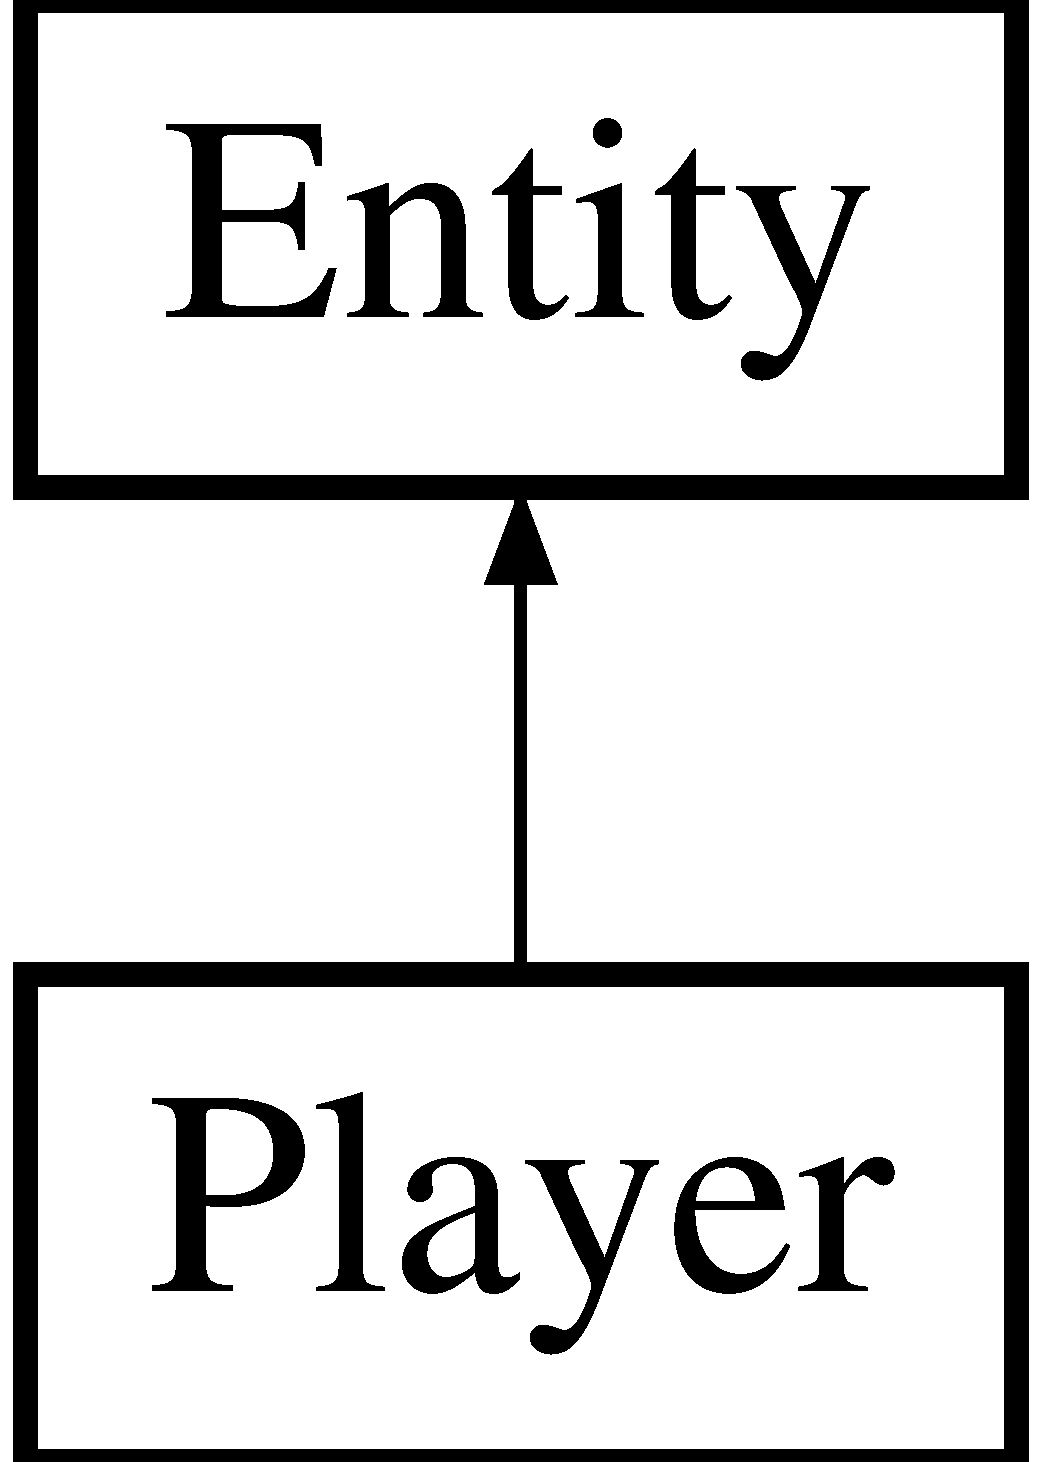
\includegraphics[height=2.000000cm]{classPlayer}
\end{center}
\end{figure}
\subsection*{Public Member Functions}
\begin{DoxyCompactItemize}
\item 
\hyperlink{classPlayer_aaa23b3bf80e8c0267cf08d4fe4d6ddc1}{Player} ()=default
\begin{DoxyCompactList}\small\item\em A default constructor. \end{DoxyCompactList}\item 
\hyperlink{classPlayer_aaaf437645956b7fd7e0acc28b64d0ae4}{Player} (unsigned int character\+\_\+id, bool is\+\_\+player1=true)
\begin{DoxyCompactList}\small\item\em Constructs a new player. \end{DoxyCompactList}\item 
void \hyperlink{classPlayer_acadddee1df9fd4fcf1a1bcca7f8b0149}{set\+Restrictions} (std\+::array$<$ int, 2 $>$ restrictions)
\begin{DoxyCompactList}\small\item\em Set restrictions in x-\/axis. \end{DoxyCompactList}\item 
void \hyperlink{classPlayer_ad3a9bf907eed07ee7ec3e2caddbb7c01}{set\+Restrictions} (int left, int right)
\begin{DoxyCompactList}\small\item\em Set restrictions in x-\/axis. \end{DoxyCompactList}\item 
void \hyperlink{classPlayer_ad61f1f07cc8e7faed52cd055a98a03d3}{set\+Start\+Position} (\hyperlink{structPoint}{Point} position)
\begin{DoxyCompactList}\small\item\em Set where player should start. \end{DoxyCompactList}\item 
void \hyperlink{classPlayer_a278252ff033b18ee6a5d9f2da5ca4fe0}{set\+Start\+Position} (int x, int y)
\begin{DoxyCompactList}\small\item\em Set where player should start. \end{DoxyCompactList}\item 
bool \hyperlink{classPlayer_a8ad2d6057db638b755b89347fbce25bb}{has\+Key} (sf\+::\+Keyboard\+::\+Key key\+\_\+code) const
\begin{DoxyCompactList}\small\item\em Checks if player has a specified key. \end{DoxyCompactList}\item 
void \hyperlink{classPlayer_a36adab5b0f1a273290786c75c280d69d}{shoot} (unsigned int projectile\+\_\+id, sf\+::\+Time current\+\_\+time)
\begin{DoxyCompactList}\small\item\em Shoots a projectile with the specified projectile id. \end{DoxyCompactList}\item 
bool \hyperlink{classPlayer_a1f5b4b98f1fa5fd8508cc2172f671b36}{ready\+To\+Use} (unsigned int projectile\+\_\+id, sf\+::\+Time current\+\_\+time)
\begin{DoxyCompactList}\small\item\em Checks if player is ready to use a projectile. \end{DoxyCompactList}\item 
void \hyperlink{classPlayer_a5fd87607be56c5175539f4e30ab09923}{remove\+Projectile} (int index)
\begin{DoxyCompactList}\small\item\em Removes a projectile for the player. \end{DoxyCompactList}\item 
bool \hyperlink{classPlayer_a5257af396fd0c0623fdf8baf0a9a634b}{collides} (\hyperlink{classProjectile}{Projectile} const \&projectile) const
\begin{DoxyCompactList}\small\item\em Checks if player collides with a projectile. \end{DoxyCompactList}\item 
void \hyperlink{classPlayer_acfc10fe38c7a5c41b201c2f29c23d544}{give\+Damage} (int amount)
\begin{DoxyCompactList}\small\item\em Damage the player. \end{DoxyCompactList}\item 
bool \hyperlink{classPlayer_a20665e4647baa8f898a62021e6204450}{is\+Dead} () const
\begin{DoxyCompactList}\small\item\em Tells if player is dead or not. \end{DoxyCompactList}\item 
void \hyperlink{classPlayer_a1af5d39f7bac2aeaa1e30c7dda2332fa}{reset} ()
\begin{DoxyCompactList}\small\item\em Reset a player. \end{DoxyCompactList}\item 
void \hyperlink{classPlayer_aa83d815158b15b6847b36c8d3473b371}{change\+State} (Player\+\_\+\+State state)
\begin{DoxyCompactList}\small\item\em Change the state of the player. \end{DoxyCompactList}\item 
Player\+\_\+\+Action \hyperlink{classPlayer_a7c1ccd08bb0263db78641f4397d5f158}{get\+Action} (sf\+::\+Keyboard\+::\+Key keycode)
\begin{DoxyCompactList}\small\item\em Get action of the player. \end{DoxyCompactList}\item 
std\+::map$<$ sf\+::\+Keyboard\+::\+Key, Player\+\_\+\+Action $>$ \hyperlink{classPlayer_af6527c6b10c6c421b07064db039c03e6}{get\+\_\+controls} () const
\begin{DoxyCompactList}\small\item\em Get player\textquotesingle{}s set controls. \end{DoxyCompactList}\item 
std\+::vector$<$ \hyperlink{classProjectile}{Projectile} $>$ \& \hyperlink{classPlayer_a0e8dc2d397dc0a6e3634cb32a01ff4cb}{get\+Active\+Projectiles} ()
\begin{DoxyCompactList}\small\item\em Get player\textquotesingle{}s shot active projectiles. \end{DoxyCompactList}\item 
std\+::vector$<$ \hyperlink{classProjectile}{Projectile} $>$ const  \& \hyperlink{classPlayer_a7593094855014964596dd9d8e6347ae6}{get\+Active\+Projectiles} () const
\begin{DoxyCompactList}\small\item\em Get player\textquotesingle{}s shot active projectiles. \end{DoxyCompactList}\item 
unsigned int \hyperlink{classPlayer_a46eff785fb376112059c90a137ac25f7}{get\+Projectile\+Id} (Projectile\+\_\+\+State const \&projectile\+\_\+state) const
\begin{DoxyCompactList}\small\item\em Get a projectile id based on projectile state. \end{DoxyCompactList}\item 
Player\+\_\+\+State \hyperlink{classPlayer_a37a57d7d3ee9e4a1a6376ac54bb71642}{get\+State} () const
\begin{DoxyCompactList}\small\item\em Get current player state. \end{DoxyCompactList}\item 
std\+::string \hyperlink{classPlayer_a6e54a09592987eef8d690ef06d815d6b}{get\+Portrait\+Source} () const
\begin{DoxyCompactList}\small\item\em Get player\textquotesingle{}s portrait source. \end{DoxyCompactList}\item 
int \hyperlink{classPlayer_ad527d6ed6e22851b0e58455ad1d602da}{get\+Current\+Health} () const
\begin{DoxyCompactList}\small\item\em Get current health. \end{DoxyCompactList}\item 
unsigned int \hyperlink{classPlayer_a367fed9b576ce0058c6f419f91ec3c7d}{get\+Max\+Health} () const
\begin{DoxyCompactList}\small\item\em Get max health. \end{DoxyCompactList}\item 
bool \hyperlink{classPlayer_ae70f285a61f1bb20d824f44cb28efa4b}{is\+Player\+One} () const
\begin{DoxyCompactList}\small\item\em Tells if player is player is player 1. \end{DoxyCompactList}\end{DoxyCompactItemize}
\subsection*{Additional Inherited Members}


\subsection{Detailed Description}
A class representing a playable character. 

An entity but with extra members needed for a playable character. 

\subsection{Constructor \& Destructor Documentation}
\mbox{\Hypertarget{classPlayer_aaa23b3bf80e8c0267cf08d4fe4d6ddc1}\label{classPlayer_aaa23b3bf80e8c0267cf08d4fe4d6ddc1}} 
\index{Player@{Player}!Player@{Player}}
\index{Player@{Player}!Player@{Player}}
\subsubsection{\texorpdfstring{Player()}{Player()}\hspace{0.1cm}{\footnotesize\ttfamily [1/2]}}
{\footnotesize\ttfamily Player\+::\+Player (\begin{DoxyParamCaption}{ }\end{DoxyParamCaption})\hspace{0.3cm}{\ttfamily [default]}}



A default constructor. 

Constructor uses compiler\textquotesingle{}s default way of constructing class. \mbox{\Hypertarget{classPlayer_aaaf437645956b7fd7e0acc28b64d0ae4}\label{classPlayer_aaaf437645956b7fd7e0acc28b64d0ae4}} 
\index{Player@{Player}!Player@{Player}}
\index{Player@{Player}!Player@{Player}}
\subsubsection{\texorpdfstring{Player()}{Player()}\hspace{0.1cm}{\footnotesize\ttfamily [2/2]}}
{\footnotesize\ttfamily Player\+::\+Player (\begin{DoxyParamCaption}\item[{unsigned int}]{character\+\_\+id,  }\item[{bool}]{is\+\_\+player1 = {\ttfamily true} }\end{DoxyParamCaption})}



Constructs a new player. 

Constructing a player with properties based on the character id and if the player is player 1 or not (else player 2) 
\begin{DoxyParams}{Parameters}
{\em character\+\_\+id} & The specified character id \\
\hline
{\em is\+\_\+player1} & If the player should be player 1 or not (else player 2) \\
\hline
\end{DoxyParams}


\subsection{Member Function Documentation}
\mbox{\Hypertarget{classPlayer_aa83d815158b15b6847b36c8d3473b371}\label{classPlayer_aa83d815158b15b6847b36c8d3473b371}} 
\index{Player@{Player}!change\+State@{change\+State}}
\index{change\+State@{change\+State}!Player@{Player}}
\subsubsection{\texorpdfstring{change\+State()}{changeState()}}
{\footnotesize\ttfamily void Player\+::change\+State (\begin{DoxyParamCaption}\item[{Player\+\_\+\+State}]{state }\end{DoxyParamCaption})}



Change the state of the player. 

Change player state of the player 
\begin{DoxyParams}{Parameters}
{\em state} & The specified player state \\
\hline
\end{DoxyParams}
\mbox{\Hypertarget{classPlayer_a5257af396fd0c0623fdf8baf0a9a634b}\label{classPlayer_a5257af396fd0c0623fdf8baf0a9a634b}} 
\index{Player@{Player}!collides@{collides}}
\index{collides@{collides}!Player@{Player}}
\subsubsection{\texorpdfstring{collides()}{collides()}}
{\footnotesize\ttfamily bool Player\+::collides (\begin{DoxyParamCaption}\item[{\hyperlink{classProjectile}{Projectile} const \&}]{projectile }\end{DoxyParamCaption}) const}



Checks if player collides with a projectile. 

Checks if player collides with a specified projectile based on position, player state and projectile state 
\begin{DoxyParams}{Parameters}
{\em projectile} & The specified projectile \\
\hline
\end{DoxyParams}
\begin{DoxyReturn}{Returns}
If player collides with the projectile or not 
\end{DoxyReturn}
\mbox{\Hypertarget{classPlayer_af6527c6b10c6c421b07064db039c03e6}\label{classPlayer_af6527c6b10c6c421b07064db039c03e6}} 
\index{Player@{Player}!get\+\_\+controls@{get\+\_\+controls}}
\index{get\+\_\+controls@{get\+\_\+controls}!Player@{Player}}
\subsubsection{\texorpdfstring{get\+\_\+controls()}{get\_controls()}}
{\footnotesize\ttfamily std\+::map$<$ sf\+::\+Keyboard\+::\+Key, Player\+\_\+\+Action $>$ Player\+::get\+\_\+controls (\begin{DoxyParamCaption}{ }\end{DoxyParamCaption}) const}



Get player\textquotesingle{}s set controls. 

Get list of controls where a keyboard key is connected to a player action \begin{DoxyReturn}{Returns}
A list of controls 
\end{DoxyReturn}
\mbox{\Hypertarget{classPlayer_a7c1ccd08bb0263db78641f4397d5f158}\label{classPlayer_a7c1ccd08bb0263db78641f4397d5f158}} 
\index{Player@{Player}!get\+Action@{get\+Action}}
\index{get\+Action@{get\+Action}!Player@{Player}}
\subsubsection{\texorpdfstring{get\+Action()}{getAction()}}
{\footnotesize\ttfamily Player\+\_\+\+Action Player\+::get\+Action (\begin{DoxyParamCaption}\item[{sf\+::\+Keyboard\+::\+Key}]{keycode }\end{DoxyParamCaption})}



Get action of the player. 

Get the player action based on the specified keyboard key. If the key was not in the set controls of the player, return player action None 
\begin{DoxyParams}{Parameters}
{\em keycode} & The specified keyboard key \\
\hline
\end{DoxyParams}
\begin{DoxyReturn}{Returns}
\hyperlink{classPlayer}{Player} action (None if key was not found) 
\end{DoxyReturn}
\mbox{\Hypertarget{classPlayer_a0e8dc2d397dc0a6e3634cb32a01ff4cb}\label{classPlayer_a0e8dc2d397dc0a6e3634cb32a01ff4cb}} 
\index{Player@{Player}!get\+Active\+Projectiles@{get\+Active\+Projectiles}}
\index{get\+Active\+Projectiles@{get\+Active\+Projectiles}!Player@{Player}}
\subsubsection{\texorpdfstring{get\+Active\+Projectiles()}{getActiveProjectiles()}\hspace{0.1cm}{\footnotesize\ttfamily [1/2]}}
{\footnotesize\ttfamily std\+::vector$<$ \hyperlink{classProjectile}{Projectile} $>$ \& Player\+::get\+Active\+Projectiles (\begin{DoxyParamCaption}{ }\end{DoxyParamCaption})}



Get player\textquotesingle{}s shot active projectiles. 

Get a reference to player\textquotesingle{}s currently active projectiles (projectiles that have been shot) \begin{DoxyReturn}{Returns}
A reference to player\textquotesingle{}s active projectiles 
\end{DoxyReturn}
\mbox{\Hypertarget{classPlayer_a7593094855014964596dd9d8e6347ae6}\label{classPlayer_a7593094855014964596dd9d8e6347ae6}} 
\index{Player@{Player}!get\+Active\+Projectiles@{get\+Active\+Projectiles}}
\index{get\+Active\+Projectiles@{get\+Active\+Projectiles}!Player@{Player}}
\subsubsection{\texorpdfstring{get\+Active\+Projectiles()}{getActiveProjectiles()}\hspace{0.1cm}{\footnotesize\ttfamily [2/2]}}
{\footnotesize\ttfamily std\+::vector$<$ \hyperlink{classProjectile}{Projectile} $>$ const  \& Player\+::get\+Active\+Projectiles (\begin{DoxyParamCaption}{ }\end{DoxyParamCaption}) const}



Get player\textquotesingle{}s shot active projectiles. 

Get an unchangeable reference to player\textquotesingle{}s currently active projectiles (projectiles that have been shot) \begin{DoxyReturn}{Returns}
An unchangeable reference to player\textquotesingle{}s active projectiles 
\end{DoxyReturn}
\mbox{\Hypertarget{classPlayer_ad527d6ed6e22851b0e58455ad1d602da}\label{classPlayer_ad527d6ed6e22851b0e58455ad1d602da}} 
\index{Player@{Player}!get\+Current\+Health@{get\+Current\+Health}}
\index{get\+Current\+Health@{get\+Current\+Health}!Player@{Player}}
\subsubsection{\texorpdfstring{get\+Current\+Health()}{getCurrentHealth()}}
{\footnotesize\ttfamily int Player\+::get\+Current\+Health (\begin{DoxyParamCaption}{ }\end{DoxyParamCaption}) const}



Get current health. 

\begin{DoxyReturn}{Returns}
The current health 
\end{DoxyReturn}
\mbox{\Hypertarget{classPlayer_a367fed9b576ce0058c6f419f91ec3c7d}\label{classPlayer_a367fed9b576ce0058c6f419f91ec3c7d}} 
\index{Player@{Player}!get\+Max\+Health@{get\+Max\+Health}}
\index{get\+Max\+Health@{get\+Max\+Health}!Player@{Player}}
\subsubsection{\texorpdfstring{get\+Max\+Health()}{getMaxHealth()}}
{\footnotesize\ttfamily unsigned int Player\+::get\+Max\+Health (\begin{DoxyParamCaption}{ }\end{DoxyParamCaption}) const}



Get max health. 

\begin{DoxyReturn}{Returns}
The max health 
\end{DoxyReturn}
\mbox{\Hypertarget{classPlayer_a6e54a09592987eef8d690ef06d815d6b}\label{classPlayer_a6e54a09592987eef8d690ef06d815d6b}} 
\index{Player@{Player}!get\+Portrait\+Source@{get\+Portrait\+Source}}
\index{get\+Portrait\+Source@{get\+Portrait\+Source}!Player@{Player}}
\subsubsection{\texorpdfstring{get\+Portrait\+Source()}{getPortraitSource()}}
{\footnotesize\ttfamily std\+::string Player\+::get\+Portrait\+Source (\begin{DoxyParamCaption}{ }\end{DoxyParamCaption}) const}



Get player\textquotesingle{}s portrait source. 

\begin{DoxyReturn}{Returns}
\hyperlink{classPlayer}{Player}\textquotesingle{}s portrait source. This is the texture to display when wanting to only show player\textquotesingle{}s face 
\end{DoxyReturn}
\mbox{\Hypertarget{classPlayer_a46eff785fb376112059c90a137ac25f7}\label{classPlayer_a46eff785fb376112059c90a137ac25f7}} 
\index{Player@{Player}!get\+Projectile\+Id@{get\+Projectile\+Id}}
\index{get\+Projectile\+Id@{get\+Projectile\+Id}!Player@{Player}}
\subsubsection{\texorpdfstring{get\+Projectile\+Id()}{getProjectileId()}}
{\footnotesize\ttfamily unsigned int Player\+::get\+Projectile\+Id (\begin{DoxyParamCaption}\item[{Projectile\+\_\+\+State const \&}]{projectile\+\_\+state }\end{DoxyParamCaption}) const}



Get a projectile id based on projectile state. 

Get a player\textquotesingle{}s projectile id based on the specified projectile state 
\begin{DoxyParams}{Parameters}
{\em projectile\+\_\+state} & Specified projectile state \\
\hline
\end{DoxyParams}
\begin{DoxyReturn}{Returns}
A projectile id with the specified projectile state 
\end{DoxyReturn}
\mbox{\Hypertarget{classPlayer_a37a57d7d3ee9e4a1a6376ac54bb71642}\label{classPlayer_a37a57d7d3ee9e4a1a6376ac54bb71642}} 
\index{Player@{Player}!get\+State@{get\+State}}
\index{get\+State@{get\+State}!Player@{Player}}
\subsubsection{\texorpdfstring{get\+State()}{getState()}}
{\footnotesize\ttfamily Player\+\_\+\+State Player\+::get\+State (\begin{DoxyParamCaption}{ }\end{DoxyParamCaption}) const}



Get current player state. 

\begin{DoxyReturn}{Returns}
Current player state 
\end{DoxyReturn}
\mbox{\Hypertarget{classPlayer_acfc10fe38c7a5c41b201c2f29c23d544}\label{classPlayer_acfc10fe38c7a5c41b201c2f29c23d544}} 
\index{Player@{Player}!give\+Damage@{give\+Damage}}
\index{give\+Damage@{give\+Damage}!Player@{Player}}
\subsubsection{\texorpdfstring{give\+Damage()}{giveDamage()}}
{\footnotesize\ttfamily void Player\+::give\+Damage (\begin{DoxyParamCaption}\item[{int}]{amount }\end{DoxyParamCaption})}



Damage the player. 

Damage player with a specified amount by decreasing player\textquotesingle{}s health 
\begin{DoxyParams}{Parameters}
{\em amount} & Amount of damage to give to player \\
\hline
\end{DoxyParams}
\mbox{\Hypertarget{classPlayer_a8ad2d6057db638b755b89347fbce25bb}\label{classPlayer_a8ad2d6057db638b755b89347fbce25bb}} 
\index{Player@{Player}!has\+Key@{has\+Key}}
\index{has\+Key@{has\+Key}!Player@{Player}}
\subsubsection{\texorpdfstring{has\+Key()}{hasKey()}}
{\footnotesize\ttfamily bool Player\+::has\+Key (\begin{DoxyParamCaption}\item[{sf\+::\+Keyboard\+::\+Key}]{key\+\_\+code }\end{DoxyParamCaption}) const}



Checks if player has a specified key. 

Checks if the specified keyboard key can be used for the player by comparing with player\textquotesingle{}s set controls 
\begin{DoxyParams}{Parameters}
{\em key\+\_\+code} & Specified keyboard key \\
\hline
\end{DoxyParams}
\begin{DoxyReturn}{Returns}
If the specified keyboard key can be used for the player 
\end{DoxyReturn}
\mbox{\Hypertarget{classPlayer_a20665e4647baa8f898a62021e6204450}\label{classPlayer_a20665e4647baa8f898a62021e6204450}} 
\index{Player@{Player}!is\+Dead@{is\+Dead}}
\index{is\+Dead@{is\+Dead}!Player@{Player}}
\subsubsection{\texorpdfstring{is\+Dead()}{isDead()}}
{\footnotesize\ttfamily bool Player\+::is\+Dead (\begin{DoxyParamCaption}{ }\end{DoxyParamCaption}) const}



Tells if player is dead or not. 

Checks if player is dead or not based on current health \begin{DoxyReturn}{Returns}
If player is dead or not 
\end{DoxyReturn}
\mbox{\Hypertarget{classPlayer_ae70f285a61f1bb20d824f44cb28efa4b}\label{classPlayer_ae70f285a61f1bb20d824f44cb28efa4b}} 
\index{Player@{Player}!is\+Player\+One@{is\+Player\+One}}
\index{is\+Player\+One@{is\+Player\+One}!Player@{Player}}
\subsubsection{\texorpdfstring{is\+Player\+One()}{isPlayerOne()}}
{\footnotesize\ttfamily bool Player\+::is\+Player\+One (\begin{DoxyParamCaption}{ }\end{DoxyParamCaption}) const}



Tells if player is player is player 1. 

Tells if the player is player 1 or not (else player 2) \begin{DoxyReturn}{Returns}
If the player is player 1 or not 
\end{DoxyReturn}
\mbox{\Hypertarget{classPlayer_a1f5b4b98f1fa5fd8508cc2172f671b36}\label{classPlayer_a1f5b4b98f1fa5fd8508cc2172f671b36}} 
\index{Player@{Player}!ready\+To\+Use@{ready\+To\+Use}}
\index{ready\+To\+Use@{ready\+To\+Use}!Player@{Player}}
\subsubsection{\texorpdfstring{ready\+To\+Use()}{readyToUse()}}
{\footnotesize\ttfamily bool Player\+::ready\+To\+Use (\begin{DoxyParamCaption}\item[{unsigned int}]{projectile\+\_\+id,  }\item[{sf\+::\+Time}]{current\+\_\+time }\end{DoxyParamCaption})}



Checks if player is ready to use a projectile. 

Checks if the projectile with the specified projectile can id is ready to use based on projectiles cooldown 
\begin{DoxyParams}{Parameters}
{\em projectile\+\_\+id} & The specified projectile id \\
\hline
{\em current\+\_\+time} & Time to compare to player\textquotesingle{}s projectile cooldowns \\
\hline
\end{DoxyParams}
\begin{DoxyReturn}{Returns}

\end{DoxyReturn}
\mbox{\Hypertarget{classPlayer_a5fd87607be56c5175539f4e30ab09923}\label{classPlayer_a5fd87607be56c5175539f4e30ab09923}} 
\index{Player@{Player}!remove\+Projectile@{remove\+Projectile}}
\index{remove\+Projectile@{remove\+Projectile}!Player@{Player}}
\subsubsection{\texorpdfstring{remove\+Projectile()}{removeProjectile()}}
{\footnotesize\ttfamily void Player\+::remove\+Projectile (\begin{DoxyParamCaption}\item[{int}]{index }\end{DoxyParamCaption})}



Removes a projectile for the player. 

Remove projectile in list of projectiles based on index 
\begin{DoxyParams}{Parameters}
{\em index} & Specified list index \\
\hline
\end{DoxyParams}
\mbox{\Hypertarget{classPlayer_a1af5d39f7bac2aeaa1e30c7dda2332fa}\label{classPlayer_a1af5d39f7bac2aeaa1e30c7dda2332fa}} 
\index{Player@{Player}!reset@{reset}}
\index{reset@{reset}!Player@{Player}}
\subsubsection{\texorpdfstring{reset()}{reset()}}
{\footnotesize\ttfamily void Player\+::reset (\begin{DoxyParamCaption}{ }\end{DoxyParamCaption})}



Reset a player. 

Resets a player by moving to start position and give player full health \mbox{\Hypertarget{classPlayer_acadddee1df9fd4fcf1a1bcca7f8b0149}\label{classPlayer_acadddee1df9fd4fcf1a1bcca7f8b0149}} 
\index{Player@{Player}!set\+Restrictions@{set\+Restrictions}}
\index{set\+Restrictions@{set\+Restrictions}!Player@{Player}}
\subsubsection{\texorpdfstring{set\+Restrictions()}{setRestrictions()}\hspace{0.1cm}{\footnotesize\ttfamily [1/2]}}
{\footnotesize\ttfamily void Player\+::set\+Restrictions (\begin{DoxyParamCaption}\item[{std\+::array$<$ int, 2 $>$}]{restrictions }\end{DoxyParamCaption})}



Set restrictions in x-\/axis. 

A player can\textquotesingle{}t move outside of the restriction. This is essentially the player\textquotesingle{}s side of the gamebaord 
\begin{DoxyParams}{Parameters}
{\em restrictions} & \\
\hline
\end{DoxyParams}
\mbox{\Hypertarget{classPlayer_ad3a9bf907eed07ee7ec3e2caddbb7c01}\label{classPlayer_ad3a9bf907eed07ee7ec3e2caddbb7c01}} 
\index{Player@{Player}!set\+Restrictions@{set\+Restrictions}}
\index{set\+Restrictions@{set\+Restrictions}!Player@{Player}}
\subsubsection{\texorpdfstring{set\+Restrictions()}{setRestrictions()}\hspace{0.1cm}{\footnotesize\ttfamily [2/2]}}
{\footnotesize\ttfamily void Player\+::set\+Restrictions (\begin{DoxyParamCaption}\item[{int}]{left,  }\item[{int}]{right }\end{DoxyParamCaption})}



Set restrictions in x-\/axis. 

A player can\textquotesingle{}t move outside of the restriction. This is essentially the player\textquotesingle{}s side of the gamebaord 
\begin{DoxyParams}{Parameters}
{\em left} & The restriction on the left side \\
\hline
{\em right} & The restriction on the right side \\
\hline
\end{DoxyParams}
\mbox{\Hypertarget{classPlayer_ad61f1f07cc8e7faed52cd055a98a03d3}\label{classPlayer_ad61f1f07cc8e7faed52cd055a98a03d3}} 
\index{Player@{Player}!set\+Start\+Position@{set\+Start\+Position}}
\index{set\+Start\+Position@{set\+Start\+Position}!Player@{Player}}
\subsubsection{\texorpdfstring{set\+Start\+Position()}{setStartPosition()}\hspace{0.1cm}{\footnotesize\ttfamily [1/2]}}
{\footnotesize\ttfamily void Player\+::set\+Start\+Position (\begin{DoxyParamCaption}\item[{\hyperlink{structPoint}{Point}}]{position }\end{DoxyParamCaption})}



Set where player should start. 


\begin{DoxyParams}{Parameters}
{\em position} & Specified position for player to start \\
\hline
\end{DoxyParams}
\mbox{\Hypertarget{classPlayer_a278252ff033b18ee6a5d9f2da5ca4fe0}\label{classPlayer_a278252ff033b18ee6a5d9f2da5ca4fe0}} 
\index{Player@{Player}!set\+Start\+Position@{set\+Start\+Position}}
\index{set\+Start\+Position@{set\+Start\+Position}!Player@{Player}}
\subsubsection{\texorpdfstring{set\+Start\+Position()}{setStartPosition()}\hspace{0.1cm}{\footnotesize\ttfamily [2/2]}}
{\footnotesize\ttfamily void Player\+::set\+Start\+Position (\begin{DoxyParamCaption}\item[{int}]{x,  }\item[{int}]{y }\end{DoxyParamCaption})}



Set where player should start. 


\begin{DoxyParams}{Parameters}
{\em x} & Where to start on x-\/axis \\
\hline
{\em y} & Where to start on y-\/axis \\
\hline
\end{DoxyParams}
\mbox{\Hypertarget{classPlayer_a36adab5b0f1a273290786c75c280d69d}\label{classPlayer_a36adab5b0f1a273290786c75c280d69d}} 
\index{Player@{Player}!shoot@{shoot}}
\index{shoot@{shoot}!Player@{Player}}
\subsubsection{\texorpdfstring{shoot()}{shoot()}}
{\footnotesize\ttfamily void Player\+::shoot (\begin{DoxyParamCaption}\item[{unsigned int}]{projectile\+\_\+id,  }\item[{sf\+::\+Time}]{current\+\_\+time }\end{DoxyParamCaption})}



Shoots a projectile with the specified projectile id. 

Shoots a projectile with a specified projectile id 
\begin{DoxyParams}{Parameters}
{\em projectile\+\_\+id} & The projectile id to shoot \\
\hline
{\em current\+\_\+time} & Time to update in player\textquotesingle{}s projectile cooldowns \\
\hline
\end{DoxyParams}


The documentation for this class was generated from the following files\+:\begin{DoxyCompactItemize}
\item 
player.\+h\item 
player.\+cpp\end{DoxyCompactItemize}

\hypertarget{structPoint}{}\section{Point Struct Reference}
\label{structPoint}\index{Point@{Point}}


Struct representing a point with an x-\/position and y-\/position.  




{\ttfamily \#include $<$struct\+\_\+point.\+h$>$}

\subsection*{Public Member Functions}
\begin{DoxyCompactItemize}
\item 
\hyperlink{structPoint_ad92f2337b839a94ce97dcdb439b4325a}{Point} ()
\begin{DoxyCompactList}\small\item\em A default contructor. \end{DoxyCompactList}\item 
\hyperlink{structPoint_acf2d96a374f9b7c9c636ba1a2ad42f02}{Point} (int \+\_\+x, int \+\_\+y)
\end{DoxyCompactItemize}
\subsection*{Public Attributes}
\begin{DoxyCompactItemize}
\item 
\mbox{\Hypertarget{structPoint_a8c779e11e694b20e0946105a9f5de842}\label{structPoint_a8c779e11e694b20e0946105a9f5de842}} 
int {\bfseries x}
\item 
\mbox{\Hypertarget{structPoint_a2e1b5fb2b2a83571f5c0bc0f66a73cf7}\label{structPoint_a2e1b5fb2b2a83571f5c0bc0f66a73cf7}} 
int {\bfseries y}
\end{DoxyCompactItemize}


\subsection{Detailed Description}
Struct representing a point with an x-\/position and y-\/position. 

\subsection{Constructor \& Destructor Documentation}
\mbox{\Hypertarget{structPoint_ad92f2337b839a94ce97dcdb439b4325a}\label{structPoint_ad92f2337b839a94ce97dcdb439b4325a}} 
\index{Point@{Point}!Point@{Point}}
\index{Point@{Point}!Point@{Point}}
\subsubsection{\texorpdfstring{Point()}{Point()}\hspace{0.1cm}{\footnotesize\ttfamily [1/2]}}
{\footnotesize\ttfamily Point\+::\+Point (\begin{DoxyParamCaption}{ }\end{DoxyParamCaption})\hspace{0.3cm}{\ttfamily [inline]}}



A default contructor. 

Sets x-\/position and y-\/position to 0 \mbox{\Hypertarget{structPoint_acf2d96a374f9b7c9c636ba1a2ad42f02}\label{structPoint_acf2d96a374f9b7c9c636ba1a2ad42f02}} 
\index{Point@{Point}!Point@{Point}}
\index{Point@{Point}!Point@{Point}}
\subsubsection{\texorpdfstring{Point()}{Point()}\hspace{0.1cm}{\footnotesize\ttfamily [2/2]}}
{\footnotesize\ttfamily Point\+::\+Point (\begin{DoxyParamCaption}\item[{int}]{\+\_\+x,  }\item[{int}]{\+\_\+y }\end{DoxyParamCaption})\hspace{0.3cm}{\ttfamily [inline]}}

Constructs a point with specified position 
\begin{DoxyParams}{Parameters}
{\em \+\_\+x} & The x-\/position \\
\hline
{\em \+\_\+y} & The y-\/position \\
\hline
\end{DoxyParams}


The documentation for this struct was generated from the following file\+:\begin{DoxyCompactItemize}
\item 
struct\+\_\+point.\+h\end{DoxyCompactItemize}

\hypertarget{classProjectile}{}\section{Projectile Class Reference}
\label{classProjectile}\index{Projectile@{Projectile}}


A class representing a shootable projectile.  




{\ttfamily \#include $<$projectile.\+h$>$}

Inheritance diagram for Projectile\+:\begin{figure}[H]
\begin{center}
\leavevmode
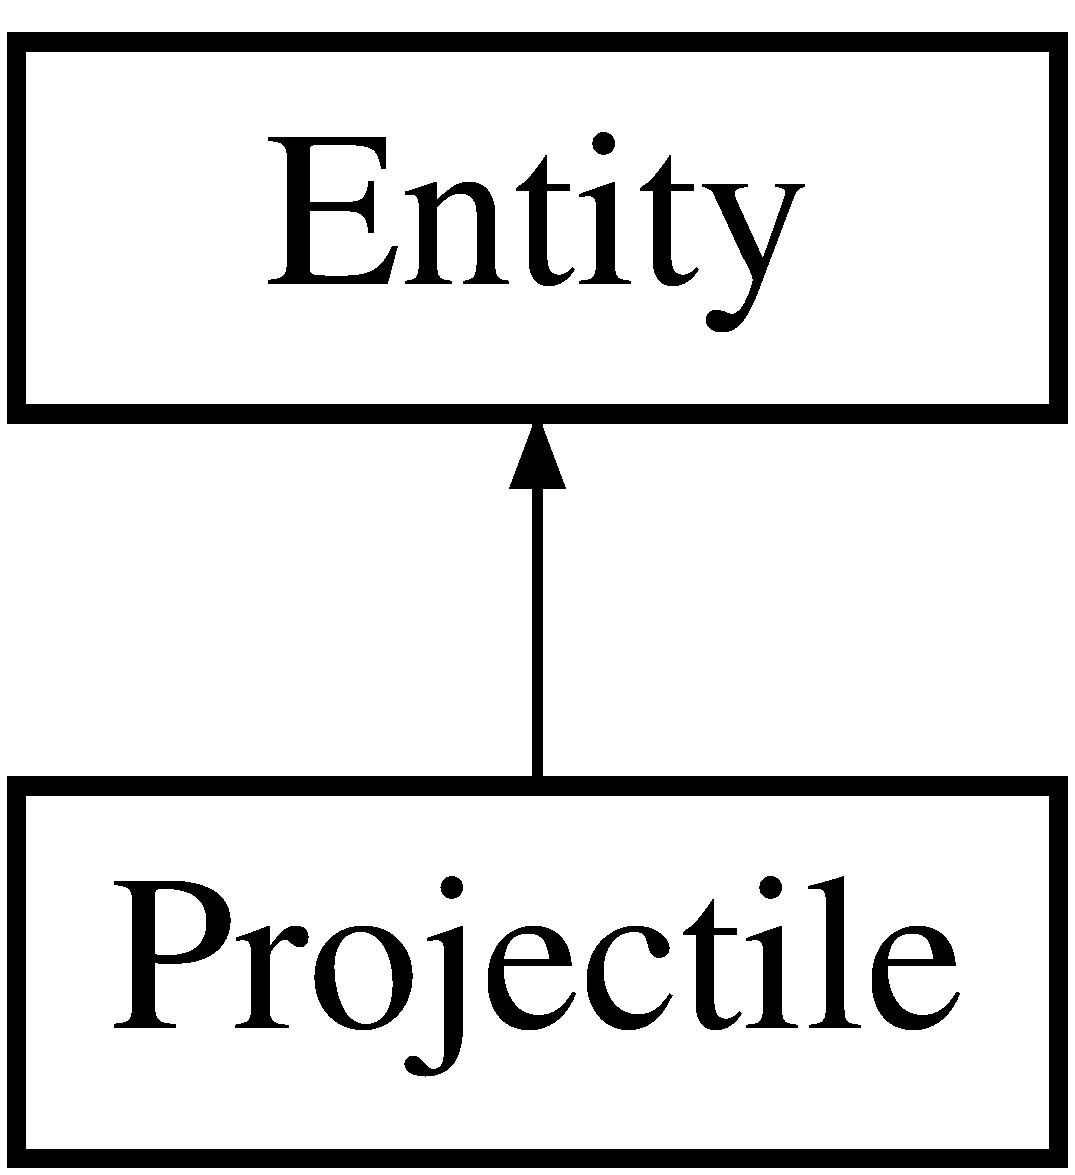
\includegraphics[height=2.000000cm]{classProjectile}
\end{center}
\end{figure}
\subsection*{Public Member Functions}
\begin{DoxyCompactItemize}
\item 
\hyperlink{classProjectile_af8b4c110af08163aeca99610e3906311}{Projectile} ()=default
\begin{DoxyCompactList}\small\item\em A default constructor. \end{DoxyCompactList}\item 
\hyperlink{classProjectile_a7b321cb748e1c2fbe83a44d4f9ec2576}{Projectile} (unsigned int projectile\+\_\+id)
\item 
bool \hyperlink{classProjectile_a54f456e92b08f461ae7410da49757f3f}{collides} (\hyperlink{classLevel}{Level} const \&level) const
\item 
void \hyperlink{classProjectile_a0ecfd73e9c4fe504f635d9b318cd241a}{change\+State} (Projectile\+\_\+\+State projectile\+\_\+state)
\item 
int \hyperlink{classProjectile_af5cd30772ad4cb3894629ca76c6b8f79}{get\+Damage} () const
\item 
double \hyperlink{classProjectile_a845770fb2b5806e1729e4bbda85849f7}{get\+Cooldown} () const
\item 
Projectile\+\_\+\+State \hyperlink{classProjectile_aa864e84b8777bed6114ef09da0c9bdad}{get\+State} () const
\begin{DoxyCompactList}\small\item\em Get the current state of the projectile. \end{DoxyCompactList}\end{DoxyCompactItemize}
\subsection*{Additional Inherited Members}


\subsection{Detailed Description}
A class representing a shootable projectile. 

An entity but with extra members needed to represent a shootable projectile 

\subsection{Constructor \& Destructor Documentation}
\mbox{\Hypertarget{classProjectile_af8b4c110af08163aeca99610e3906311}\label{classProjectile_af8b4c110af08163aeca99610e3906311}} 
\index{Projectile@{Projectile}!Projectile@{Projectile}}
\index{Projectile@{Projectile}!Projectile@{Projectile}}
\subsubsection{\texorpdfstring{Projectile()}{Projectile()}\hspace{0.1cm}{\footnotesize\ttfamily [1/2]}}
{\footnotesize\ttfamily Projectile\+::\+Projectile (\begin{DoxyParamCaption}{ }\end{DoxyParamCaption})\hspace{0.3cm}{\ttfamily [default]}}



A default constructor. 

Constructor uses compiler\textquotesingle{}s default way of constructing class. \mbox{\Hypertarget{classProjectile_a7b321cb748e1c2fbe83a44d4f9ec2576}\label{classProjectile_a7b321cb748e1c2fbe83a44d4f9ec2576}} 
\index{Projectile@{Projectile}!Projectile@{Projectile}}
\index{Projectile@{Projectile}!Projectile@{Projectile}}
\subsubsection{\texorpdfstring{Projectile()}{Projectile()}\hspace{0.1cm}{\footnotesize\ttfamily [2/2]}}
{\footnotesize\ttfamily Projectile\+::\+Projectile (\begin{DoxyParamCaption}\item[{unsigned int}]{projectile\+\_\+id }\end{DoxyParamCaption})}

Constructing a projectile with properties based on the projectile id 
\begin{DoxyParams}{Parameters}
{\em projectile\+\_\+id} & The specified projectile id \\
\hline
\end{DoxyParams}


\subsection{Member Function Documentation}
\mbox{\Hypertarget{classProjectile_a0ecfd73e9c4fe504f635d9b318cd241a}\label{classProjectile_a0ecfd73e9c4fe504f635d9b318cd241a}} 
\index{Projectile@{Projectile}!change\+State@{change\+State}}
\index{change\+State@{change\+State}!Projectile@{Projectile}}
\subsubsection{\texorpdfstring{change\+State()}{changeState()}}
{\footnotesize\ttfamily void Projectile\+::change\+State (\begin{DoxyParamCaption}\item[{Projectile\+\_\+\+State}]{projectile\+\_\+state }\end{DoxyParamCaption})}

Change the projectile state of the projectile 
\begin{DoxyParams}{Parameters}
{\em projectile\+\_\+state} & The specfied projectile state \\
\hline
\end{DoxyParams}
\mbox{\Hypertarget{classProjectile_a54f456e92b08f461ae7410da49757f3f}\label{classProjectile_a54f456e92b08f461ae7410da49757f3f}} 
\index{Projectile@{Projectile}!collides@{collides}}
\index{collides@{collides}!Projectile@{Projectile}}
\subsubsection{\texorpdfstring{collides()}{collides()}}
{\footnotesize\ttfamily bool Projectile\+::collides (\begin{DoxyParamCaption}\item[{\hyperlink{classLevel}{Level} const \&}]{level }\end{DoxyParamCaption}) const}

Checks if the projectile collides with the specified level or not. This is done by comparing position of projectile with width and height of the level. 
\begin{DoxyParams}{Parameters}
{\em level} & The specified level \\
\hline
\end{DoxyParams}
\begin{DoxyReturn}{Returns}
If the projectile collides with the specified level or not 
\end{DoxyReturn}
\mbox{\Hypertarget{classProjectile_a845770fb2b5806e1729e4bbda85849f7}\label{classProjectile_a845770fb2b5806e1729e4bbda85849f7}} 
\index{Projectile@{Projectile}!get\+Cooldown@{get\+Cooldown}}
\index{get\+Cooldown@{get\+Cooldown}!Projectile@{Projectile}}
\subsubsection{\texorpdfstring{get\+Cooldown()}{getCooldown()}}
{\footnotesize\ttfamily double Projectile\+::get\+Cooldown (\begin{DoxyParamCaption}{ }\end{DoxyParamCaption}) const}

Get the cooldown of the projectile \begin{DoxyReturn}{Returns}
The cooldown of the projectile 
\end{DoxyReturn}
\mbox{\Hypertarget{classProjectile_af5cd30772ad4cb3894629ca76c6b8f79}\label{classProjectile_af5cd30772ad4cb3894629ca76c6b8f79}} 
\index{Projectile@{Projectile}!get\+Damage@{get\+Damage}}
\index{get\+Damage@{get\+Damage}!Projectile@{Projectile}}
\subsubsection{\texorpdfstring{get\+Damage()}{getDamage()}}
{\footnotesize\ttfamily int Projectile\+::get\+Damage (\begin{DoxyParamCaption}{ }\end{DoxyParamCaption}) const}

Get the damage of the projectile \begin{DoxyReturn}{Returns}
The damage of the projectile 
\end{DoxyReturn}
\mbox{\Hypertarget{classProjectile_aa864e84b8777bed6114ef09da0c9bdad}\label{classProjectile_aa864e84b8777bed6114ef09da0c9bdad}} 
\index{Projectile@{Projectile}!get\+State@{get\+State}}
\index{get\+State@{get\+State}!Projectile@{Projectile}}
\subsubsection{\texorpdfstring{get\+State()}{getState()}}
{\footnotesize\ttfamily Projectile\+\_\+\+State Projectile\+::get\+State (\begin{DoxyParamCaption}{ }\end{DoxyParamCaption}) const}



Get the current state of the projectile. 

Get the current state of the projectile \begin{DoxyReturn}{Returns}
The current state of the projectile 
\end{DoxyReturn}


The documentation for this class was generated from the following files\+:\begin{DoxyCompactItemize}
\item 
projectile.\+h\item 
projectile.\+cpp\end{DoxyCompactItemize}

\hypertarget{classWinning__Window}{}\section{Winning\+\_\+\+Window Class Reference}
\label{classWinning__Window}\index{Winning\+\_\+\+Window@{Winning\+\_\+\+Window}}


A class representing a winning window.  




{\ttfamily \#include $<$winning\+\_\+window.\+h$>$}

Inheritance diagram for Winning\+\_\+\+Window\+:\begin{figure}[H]
\begin{center}
\leavevmode
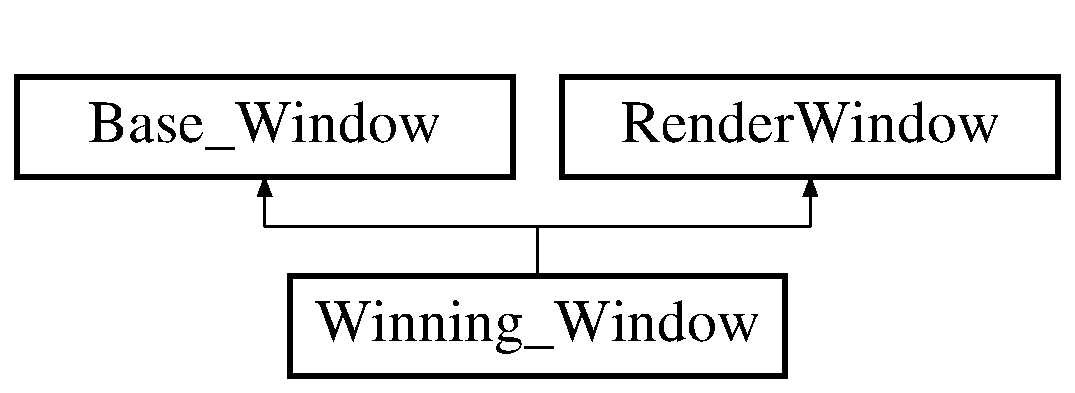
\includegraphics[height=2.000000cm]{classWinning__Window}
\end{center}
\end{figure}
\subsection*{Public Member Functions}
\begin{DoxyCompactItemize}
\item 
\hyperlink{classWinning__Window_adc2ffaa54ae59ffd3f50611dac1537b1}{Winning\+\_\+\+Window} ()=default
\begin{DoxyCompactList}\small\item\em A default constructor. \end{DoxyCompactList}\item 
void \hyperlink{classWinning__Window_a3382d7cac361e9909851407bf27efa58}{initialize} (\hyperlink{classPlayer}{Player} const \&winner_text)
\begin{DoxyCompactList}\small\item\em Initializes member variables of the winning window. \end{DoxyCompactList}\item 
void \hyperlink{classWinning__Window_a6daa7eec7198015a1f154cc9cb9b22c5}{update\+Graphics} ()
\begin{DoxyCompactList}\small\item\em Update graphical display of the gameboard window. \end{DoxyCompactList}\item 
void \hyperlink{classWinning__Window_a93f258448a7ab61ec6931e7bfb25b614}{go\+Up} ()
\begin{DoxyCompactList}\small\item\em Go up in the winning menu. \end{DoxyCompactList}\item 
void \hyperlink{classWinning__Window_ac6d149dfb7cd9c8978117eecd70a3923}{go\+Down} ()
\begin{DoxyCompactList}\small\item\em Go up in the winning menu. \end{DoxyCompactList}\item 
Winning\+\_\+\+Option \hyperlink{classWinning__Window_aaa8755d6751054b38c9eb3b085db4fdf}{get\+Winning\+Option} ()
\begin{DoxyCompactList}\small\item\em Get user\textquotesingle{}s currently selected winning choice. \end{DoxyCompactList}\end{DoxyCompactItemize}
\subsection*{Additional Inherited Members}


\subsection{Detailed Description}
A class representing a winning window. 

A class inheriting from \char`\"{}\+Base\+\_\+\+Window\char`\"{} to make class represent a window. In addition the class contains members needed for a winning window in the game. A winning window is the window that should appear after a match is finished. The window shows who has won and let player\textquotesingle{}s select what do after the match. 

\subsection{Constructor \& Destructor Documentation}
\mbox{\Hypertarget{classWinning__Window_adc2ffaa54ae59ffd3f50611dac1537b1}\label{classWinning__Window_adc2ffaa54ae59ffd3f50611dac1537b1}} 
\index{Winning\+\_\+\+Window@{Winning\+\_\+\+Window}!Winning\+\_\+\+Window@{Winning\+\_\+\+Window}}
\index{Winning\+\_\+\+Window@{Winning\+\_\+\+Window}!Winning\+\_\+\+Window@{Winning\+\_\+\+Window}}
\subsubsection{\texorpdfstring{Winning\+\_\+\+Window()}{Winning\_Window()}}
{\footnotesize\ttfamily Winning\+\_\+\+Window\+::\+Winning\+\_\+\+Window (\begin{DoxyParamCaption}{ }\end{DoxyParamCaption})\hspace{0.3cm}{\ttfamily [default]}}



A default constructor. 

Constructor uses compiler\textquotesingle{}s default way of constructing class. 

\subsection{Member Function Documentation}
\mbox{\Hypertarget{classWinning__Window_aaa8755d6751054b38c9eb3b085db4fdf}\label{classWinning__Window_aaa8755d6751054b38c9eb3b085db4fdf}} 
\index{Winning\+\_\+\+Window@{Winning\+\_\+\+Window}!get\+Winning\+Option@{get\+Winning\+Option}}
\index{get\+Winning\+Option@{get\+Winning\+Option}!Winning\+\_\+\+Window@{Winning\+\_\+\+Window}}
\subsubsection{\texorpdfstring{get\+Winning\+Option()}{getWinningOption()}}
{\footnotesize\ttfamily Winning\+\_\+\+Option Winning\+\_\+\+Window\+::get\+Winning\+Option (\begin{DoxyParamCaption}{ }\end{DoxyParamCaption})}



Get user\textquotesingle{}s currently selected winning choice. 

\begin{DoxyReturn}{Returns}
The selected wining option 
\end{DoxyReturn}
\mbox{\Hypertarget{classWinning__Window_ac6d149dfb7cd9c8978117eecd70a3923}\label{classWinning__Window_ac6d149dfb7cd9c8978117eecd70a3923}} 
\index{Winning\+\_\+\+Window@{Winning\+\_\+\+Window}!go\+Down@{go\+Down}}
\index{go\+Down@{go\+Down}!Winning\+\_\+\+Window@{Winning\+\_\+\+Window}}
\subsubsection{\texorpdfstring{go\+Down()}{goDown()}}
{\footnotesize\ttfamily void Winning\+\_\+\+Window\+::go\+Down (\begin{DoxyParamCaption}{ }\end{DoxyParamCaption})}



Go up in the winning menu. 

Go down in the selectable winning options \mbox{\Hypertarget{classWinning__Window_a93f258448a7ab61ec6931e7bfb25b614}\label{classWinning__Window_a93f258448a7ab61ec6931e7bfb25b614}} 
\index{Winning\+\_\+\+Window@{Winning\+\_\+\+Window}!go\+Up@{go\+Up}}
\index{go\+Up@{go\+Up}!Winning\+\_\+\+Window@{Winning\+\_\+\+Window}}
\subsubsection{\texorpdfstring{go\+Up()}{goUp()}}
{\footnotesize\ttfamily void Winning\+\_\+\+Window\+::go\+Up (\begin{DoxyParamCaption}{ }\end{DoxyParamCaption})}



Go up in the winning menu. 

Go up in the selectable winning options \mbox{\Hypertarget{classWinning__Window_a3382d7cac361e9909851407bf27efa58}\label{classWinning__Window_a3382d7cac361e9909851407bf27efa58}} 
\index{Winning\+\_\+\+Window@{Winning\+\_\+\+Window}!initialize@{initialize}}
\index{initialize@{initialize}!Winning\+\_\+\+Window@{Winning\+\_\+\+Window}}
\subsubsection{\texorpdfstring{initialize()}{initialize()}}
{\footnotesize\ttfamily void Winning\+\_\+\+Window\+::initialize (\begin{DoxyParamCaption}\item[{\hyperlink{classPlayer}{Player} const \&}]{winner_text }\end{DoxyParamCaption})}



Initializes member variables of the winning window. 

Initializes member variables of the winning window based on who is the winner_text \mbox{\Hypertarget{classWinning__Window_a6daa7eec7198015a1f154cc9cb9b22c5}\label{classWinning__Window_a6daa7eec7198015a1f154cc9cb9b22c5}}
\index{Winning\+\_\+\+Window@{Winning\+\_\+\+Window}!update\+Graphics@{update\+Graphics}}
\index{update\+Graphics@{update\+Graphics}!Winning\+\_\+\+Window@{Winning\+\_\+\+Window}}
\subsubsection{\texorpdfstring{update\+Graphics()}{updateGraphics()}}
{\footnotesize\ttfamily void Winning\+\_\+\+Window\+::update\+Graphics (\begin{DoxyParamCaption}{ }\end{DoxyParamCaption})}



Update graphical display of the gameboard window. 

Member function to update the graphics of the window based on possible changes 

The documentation for this class was generated from the following files\+:\begin{DoxyCompactItemize}
\item 
winning\+\_\+window.\+h\item 
winning\+\_\+window.\+cpp\end{DoxyCompactItemize}

%--- End generated contents ---

% Index
\backmatter
\newpage
\phantomsection
\clearemptydoublepage
\addcontentsline{toc}{chapter}{Index}
\printindex

\end{document}
